\documentclass[]{article}
\usepackage{lmodern}
\usepackage{amssymb,amsmath}
\usepackage{ifxetex,ifluatex}
\usepackage{fixltx2e} % provides \textsubscript
\ifnum 0\ifxetex 1\fi\ifluatex 1\fi=0 % if pdftex
  \usepackage[T1]{fontenc}
  \usepackage[utf8]{inputenc}
\else % if luatex or xelatex
  \ifxetex
    \usepackage{mathspec}
  \else
    \usepackage{fontspec}
  \fi
  \defaultfontfeatures{Ligatures=TeX,Scale=MatchLowercase}
\fi
% use upquote if available, for straight quotes in verbatim environments
\IfFileExists{upquote.sty}{\usepackage{upquote}}{}
% use microtype if available
\IfFileExists{microtype.sty}{%
\usepackage{microtype}
\UseMicrotypeSet[protrusion]{basicmath} % disable protrusion for tt fonts
}{}
\usepackage[margin=1in]{geometry}
\usepackage{hyperref}
\hypersetup{unicode=true,
            pdftitle={Laborator 3},
            pdfborder={0 0 0},
            breaklinks=true}
\urlstyle{same}  % don't use monospace font for urls
\usepackage{color}
\usepackage{fancyvrb}
\newcommand{\VerbBar}{|}
\newcommand{\VERB}{\Verb[commandchars=\\\{\}]}
\DefineVerbatimEnvironment{Highlighting}{Verbatim}{commandchars=\\\{\}}
% Add ',fontsize=\small' for more characters per line
\usepackage{framed}
\definecolor{shadecolor}{RGB}{248,248,248}
\newenvironment{Shaded}{\begin{snugshade}}{\end{snugshade}}
\newcommand{\KeywordTok}[1]{\textcolor[rgb]{0.13,0.29,0.53}{\textbf{#1}}}
\newcommand{\DataTypeTok}[1]{\textcolor[rgb]{0.13,0.29,0.53}{#1}}
\newcommand{\DecValTok}[1]{\textcolor[rgb]{0.00,0.00,0.81}{#1}}
\newcommand{\BaseNTok}[1]{\textcolor[rgb]{0.00,0.00,0.81}{#1}}
\newcommand{\FloatTok}[1]{\textcolor[rgb]{0.00,0.00,0.81}{#1}}
\newcommand{\ConstantTok}[1]{\textcolor[rgb]{0.00,0.00,0.00}{#1}}
\newcommand{\CharTok}[1]{\textcolor[rgb]{0.31,0.60,0.02}{#1}}
\newcommand{\SpecialCharTok}[1]{\textcolor[rgb]{0.00,0.00,0.00}{#1}}
\newcommand{\StringTok}[1]{\textcolor[rgb]{0.31,0.60,0.02}{#1}}
\newcommand{\VerbatimStringTok}[1]{\textcolor[rgb]{0.31,0.60,0.02}{#1}}
\newcommand{\SpecialStringTok}[1]{\textcolor[rgb]{0.31,0.60,0.02}{#1}}
\newcommand{\ImportTok}[1]{#1}
\newcommand{\CommentTok}[1]{\textcolor[rgb]{0.56,0.35,0.01}{\textit{#1}}}
\newcommand{\DocumentationTok}[1]{\textcolor[rgb]{0.56,0.35,0.01}{\textbf{\textit{#1}}}}
\newcommand{\AnnotationTok}[1]{\textcolor[rgb]{0.56,0.35,0.01}{\textbf{\textit{#1}}}}
\newcommand{\CommentVarTok}[1]{\textcolor[rgb]{0.56,0.35,0.01}{\textbf{\textit{#1}}}}
\newcommand{\OtherTok}[1]{\textcolor[rgb]{0.56,0.35,0.01}{#1}}
\newcommand{\FunctionTok}[1]{\textcolor[rgb]{0.00,0.00,0.00}{#1}}
\newcommand{\VariableTok}[1]{\textcolor[rgb]{0.00,0.00,0.00}{#1}}
\newcommand{\ControlFlowTok}[1]{\textcolor[rgb]{0.13,0.29,0.53}{\textbf{#1}}}
\newcommand{\OperatorTok}[1]{\textcolor[rgb]{0.81,0.36,0.00}{\textbf{#1}}}
\newcommand{\BuiltInTok}[1]{#1}
\newcommand{\ExtensionTok}[1]{#1}
\newcommand{\PreprocessorTok}[1]{\textcolor[rgb]{0.56,0.35,0.01}{\textit{#1}}}
\newcommand{\AttributeTok}[1]{\textcolor[rgb]{0.77,0.63,0.00}{#1}}
\newcommand{\RegionMarkerTok}[1]{#1}
\newcommand{\InformationTok}[1]{\textcolor[rgb]{0.56,0.35,0.01}{\textbf{\textit{#1}}}}
\newcommand{\WarningTok}[1]{\textcolor[rgb]{0.56,0.35,0.01}{\textbf{\textit{#1}}}}
\newcommand{\AlertTok}[1]{\textcolor[rgb]{0.94,0.16,0.16}{#1}}
\newcommand{\ErrorTok}[1]{\textcolor[rgb]{0.64,0.00,0.00}{\textbf{#1}}}
\newcommand{\NormalTok}[1]{#1}
\usepackage{graphicx,grffile}
\makeatletter
\def\maxwidth{\ifdim\Gin@nat@width>\linewidth\linewidth\else\Gin@nat@width\fi}
\def\maxheight{\ifdim\Gin@nat@height>\textheight\textheight\else\Gin@nat@height\fi}
\makeatother
% Scale images if necessary, so that they will not overflow the page
% margins by default, and it is still possible to overwrite the defaults
% using explicit options in \includegraphics[width, height, ...]{}
\setkeys{Gin}{width=\maxwidth,height=\maxheight,keepaspectratio}
\IfFileExists{parskip.sty}{%
\usepackage{parskip}
}{% else
\setlength{\parindent}{0pt}
\setlength{\parskip}{6pt plus 2pt minus 1pt}
}
\setlength{\emergencystretch}{3em}  % prevent overfull lines
\providecommand{\tightlist}{%
  \setlength{\itemsep}{0pt}\setlength{\parskip}{0pt}}
\setcounter{secnumdepth}{5}
% Redefines (sub)paragraphs to behave more like sections
\ifx\paragraph\undefined\else
\let\oldparagraph\paragraph
\renewcommand{\paragraph}[1]{\oldparagraph{#1}\mbox{}}
\fi
\ifx\subparagraph\undefined\else
\let\oldsubparagraph\subparagraph
\renewcommand{\subparagraph}[1]{\oldsubparagraph{#1}\mbox{}}
\fi

%%% Use protect on footnotes to avoid problems with footnotes in titles
\let\rmarkdownfootnote\footnote%
\def\footnote{\protect\rmarkdownfootnote}

%%% Change title format to be more compact
\usepackage{titling}

% Create subtitle command for use in maketitle
\newcommand{\subtitle}[1]{
  \posttitle{
    \begin{center}\large#1\end{center}
    }
}

\setlength{\droptitle}{-2em}
  \title{Laborator 3}
  \pretitle{\vspace{\droptitle}\centering\huge}
  \posttitle{\par}
\subtitle{Elemente de statistică descriptivă}
  \author{}
  \preauthor{}\postauthor{}
  \date{}
  \predate{}\postdate{}

\usepackage{booktabs}
\usepackage{longtable}
\usepackage{framed,color}
\definecolor{shadecolor}{RGB}{248, 248, 248}
%\definecolor{shadecolor1}{RGB}{216,225,235}
%\definecolor{framecolor}{RGB}{108,123,13}

%\definecolor{shadecolor}{RGB}{226, 255, 241}
\definecolor{shadecolor1}{RGB}{217,225,199}
\definecolor{framecolor}{RGB}{60,179,113}

\ifxetex
  \usepackage{letltxmacro}
  \setlength{\XeTeXLinkMargin}{1pt}
  \LetLtxMacro\SavedIncludeGraphics\includegraphics
  \def\includegraphics#1#{% #1 catches optional stuff (star/opt. arg.)
    \IncludeGraphicsAux{#1}%
  }%
  \newcommand*{\IncludeGraphicsAux}[2]{%
    \XeTeXLinkBox{%
      \SavedIncludeGraphics#1{#2}%
    }%
  }%
\fi

\newenvironment{frshaded*}{%
  \def\FrameCommand{\fboxrule=\FrameRule\fboxsep=\FrameSep \fcolorbox{framecolor}{shadecolor1}}%
  \MakeFramed {\advance\hsize-\width \FrameRestore}}%
{\endMakeFramed}

\newenvironment{rmdblock}[1]
  {\begin{frshaded*}
  \begin{itemize}
  \renewcommand{\labelitemi}{
    \raisebox{-.7\height}[0pt][0pt]{
      {\setkeys{Gin}{width=2em,keepaspectratio}\includegraphics{images/icons/#1}}
    }
  }
  \item
  }
  {
  \end{itemize}
  \end{frshaded*}
  }

\newenvironment{rmdcaution}
  {\begin{rmdblock}{caution}}
  {\end{rmdblock}}
% \newenvironment{rmdinsight}
%   {\begin{rmdblock}{insight}}
%   {\end{rmdblock}}
\newenvironment{rmdexercise}
  {\begin{rmdblock}{exercise}}
  {\end{rmdblock}}
\newenvironment{rmdtip}
  {\begin{rmdblock}{tip}}
  {\end{rmdblock}}


%%%%%%%%%%%%%%%%%%%%%%%%%%%%%%%%%%%%%%%%%%%%%%%%%%%%%%%%%%%%%%%%%%%%%%%%%%%%%%%%%%%%%%%%%%%%%%%%%%%%%%%%%%%%%%%%%%%%%
%%%%%%%%%%% For insight block %%%%%%%%%%%%%%%%%%%%%%%%%%
\definecolor{shadecolor_insight}{RGB}{223,240,216}
\definecolor{framecolor_insight}{RGB}{136,193,137}

%\definecolor{shadecolor_insight}{RGB}{217,225,199}
%\definecolor{framecolor_insight}{RGB}{60,179,113}

\newenvironment{frshaded_insight*}{%
  \def\FrameCommand{\fboxrule=\FrameRule\fboxsep=\FrameSep \fcolorbox{framecolor_insight}{shadecolor_insight}}%
  \MakeFramed {\advance\hsize-\width \FrameRestore}}%
{\endMakeFramed}

\newenvironment{rmdblock_insight}[1]
  {\begin{frshaded_insight*}
  \begin{itemize}
  \renewcommand{\labelitemi}{
    \raisebox{-.7\height}[0pt][0pt]{
      {\setkeys{Gin}{width=2em,keepaspectratio}\includegraphics{images/icons/#1}}
    }
  }
  \item
  }
  {
  \end{itemize}
  \end{frshaded_insight*}
  }

\newenvironment{rmdinsight}
  {\begin{rmdblock_insight}{insight}}
  {\end{rmdblock_insight}}

%%%%%%%%%%%%%%%%%%%%%%%%%%%%%%%%%%%%%%%%%%%%%%%%%%%%%%%%%%%%%%%%%%%%%%%%%%%%%%%%%%%%%%%%%%%%%%%%%%%%%%%%%%%%%%%%%%%%%
\usepackage{subfigure}
\usepackage{booktabs}
\usepackage{slashbox}
\usepackage{color}
%%%%%%%%%%%%%%%%%%%%%%%%%%%%%%%%%%%%%%%%%%%%%%%%%%%%%%%%%%%%%%%%%%%%%%%%%%%%%%%%%%%%%%%%%%%%%%%%%%%%%%%%%%%%%%%%%%%%%
%CITEVA DEFINITII
\def\om{\omega}
\def\Om{\Omega}
\def\et{\eta}
\def\td{\tilde{\delta}}
\def\m{{\mu}}
\def\n{{\nu}}
\def\k{{\kappa}}
\def\l{{\lambda}}
\def\L{{\Lambda}}
\def\g{{\gamma}}
\def\a{{\alpha}}
\def\e{{\varepsilon}}
\def\b{{\beta}}
\def\G{{\Gamma}}
\def\d{{\delta}}
\def\D{{\Delta}}
\def\t{{\theta}}
\def\s{{\sigma}}
\def\S{{\Sigma}}
\def\z{{\zeta}}
\def\qed{\hfill\Box}
\def\ds{\displaystyle}
\def\mc{\mathcal}
%%%%%%%%%%%%%%%%%%%%%%%%%%%%%%%%%%%%%%%%%%%%%%%%%%%%%%%%%%%%%%%%%%%%%%%%%%%%%%%%%%%%%%%%%%%%%%%%%%%%%%%%%%%%%%%%%%%%%%
\def\1{{\mathbf 1}}
\def\CC{{\mathbb C}}
\def\VV{{\mathbb V}}
\def\RR{{\mathbb R}}
\def\QQ{{\mathbb Q}}
\def\ZZ{{\mathbb Z}}
\def\PP{{\mathbb P}}
\def\EE{{\mathbb E}}
\def\NN{{\mathbb N}}
\def\FF{{\mathbb F}}
%\def\SS{{\mathbb S}}
\def\MA{{\mathcal A}}
\def\MO{{\mathcal O}}
\def\MF{{\mathcal F}}
\def\ME{{\mathcal E}}
\def\MR{{\mathcal R}}
\def\MB{{\mathcal B}}
\def\MM{{\mathcal M}}
\def\MN{{\mathcal N}}
\def\MU{{\mathcal U}}
\def\MP{{\mathcal P}}
\def\MS{{\mathcal S}}
\def\MBS{{\mathbf S}}
\def\MX{{\bm{ \mathscr X}}}

% independent sign
\newcommand\independent{\protect\mathpalette{\protect\independenT}{\perp}}
\def\independenT#1#2{\mathrel{\rlap{$#1#2$}\mkern2mu{#1#2}}}

\renewcommand\tablename{Tab.}
\renewcommand{\figurename}{Fig.}
\renewcommand\refname{Referințe}

%%%%%%%%%%%%%%%%%%%%%%%%%%%%%%%%%%%%%%%%%%%%%%%%%%%%%%%%%%%%%%%%%%%%%%%%%%%%%%%%%%%%%%%%%%%%%%%%%%%%%%%%%%%%%%%%%%%%%
%Header and Footer
\usepackage{fancyhdr}

\pagestyle{fancy}
\fancyhf{}
\rhead{Universitatea din Bucure\c sti\\ Facultatea de Matematic\u a \c si Informatic\u a}
\lhead{\textit{Curs}: Instrumente Statistice pentru Finan\c te\\ \textit{Instructor}: A. Am\u arioarei}
\rfoot{Pagina \thepage}
\lfoot{Grupa: 403}
%%%%%%%%%%%%%%%%%%%%%%%%%%%%%%%%%%%%%%%
\usepackage{booktabs}
\usepackage{longtable}
\usepackage{array}
\usepackage{multirow}
\usepackage[table]{xcolor}
\usepackage{wrapfig}
\usepackage{float}
\usepackage{colortbl}
\usepackage{pdflscape}
\usepackage{tabu}
\usepackage{threeparttable}
\usepackage[normalem]{ulem}

\begin{document}
\maketitle

%%%%%%%%%%%%%%%%%%%%%%%%
\thispagestyle{fancy}

Obiectivul acestui laborator este de a prezenta câteva elemente
(numerice și grafice) de statistică descriptivă/exploratorie pentru
studiul rentabilității zilnice (\emph{daily returns}) a unui număr de
active reprezentative (assets).

\section{Importarea datelor}\label{importarea-datelor}

Înainte de a analiza datele trebuie să le descărcăm și să le punem
într-un format ușor de utilizat pentru analiză. Datele pot fi obținute
de pe diferite platforme online precum
\href{https://finance.yahoo.com/}{Yahoo!Finance} sau
\href{https://finance.google.com/finance}{Google Finance}. Mai jos este
ilustrat codul funcției \texttt{google\_stocks} care permite extragerea
datelor de pe platforma \href{https://finance.google.com/finance}{Google
Finance}:

\begin{Shaded}
\begin{Highlighting}[]
\NormalTok{google_stocks <-}\StringTok{ }\ControlFlowTok{function}\NormalTok{(sym, }\DataTypeTok{current =} \OtherTok{TRUE}\NormalTok{, }\DataTypeTok{sy =} \DecValTok{2007}\NormalTok{, }\DataTypeTok{sm =} \DecValTok{1}\NormalTok{, }\DataTypeTok{sd =} \DecValTok{1}\NormalTok{, ey, em, ed)}
\NormalTok{\{}
  \CommentTok{# sy, sm, sd, ey, em, ed corespund la}
  \CommentTok{# start year, start month, start day, end year, end month, si end day}
  
  \CommentTok{# Daca este TRUE folosim data curenta}
  \ControlFlowTok{if}\NormalTok{(current)\{}
\NormalTok{    system_time <-}\StringTok{ }\KeywordTok{as.character}\NormalTok{(}\KeywordTok{Sys.time}\NormalTok{())}
\NormalTok{    ey <-}\StringTok{ }\KeywordTok{as.numeric}\NormalTok{(}\KeywordTok{substr}\NormalTok{(system_time, }\DataTypeTok{start =} \DecValTok{1}\NormalTok{, }\DataTypeTok{stop =} \DecValTok{4}\NormalTok{))}
\NormalTok{    em <-}\StringTok{ }\KeywordTok{as.numeric}\NormalTok{(}\KeywordTok{substr}\NormalTok{(system_time, }\DataTypeTok{start =} \DecValTok{6}\NormalTok{, }\DataTypeTok{stop =} \DecValTok{7}\NormalTok{))}
\NormalTok{    ed <-}\StringTok{ }\KeywordTok{as.numeric}\NormalTok{(}\KeywordTok{substr}\NormalTok{(system_time, }\DataTypeTok{start =} \DecValTok{9}\NormalTok{, }\DataTypeTok{stop =} \DecValTok{10}\NormalTok{))}
\NormalTok{  \}}

\NormalTok{  tmp <-}\StringTok{ }\KeywordTok{tempfile}\NormalTok{()}
  
  \CommentTok{# cat("downloading ", sym, ".....\textbackslash{}n\textbackslash{}n")}
\NormalTok{  google.URL =}\StringTok{ "http://finance.google.com/finance/historical?"}
  \KeywordTok{download.file}\NormalTok{(}\KeywordTok{paste}\NormalTok{(google.URL, }\StringTok{"q="}\NormalTok{, sym, }\StringTok{"&startdate="}\NormalTok{, }
\NormalTok{                      month.abb[sm], }\StringTok{"+"}\NormalTok{, }\KeywordTok{sprintf}\NormalTok{(}\StringTok{"%.2d"}\NormalTok{, sd), }
                      \StringTok{",+"}\NormalTok{, sy, }\StringTok{"&enddate="}\NormalTok{, month.abb[em], }\StringTok{"+"}\NormalTok{, }
                      \KeywordTok{sprintf}\NormalTok{(}\StringTok{"%.2d"}\NormalTok{, ed), }\StringTok{",+"}\NormalTok{, ey, }\StringTok{"&output=csv"}\NormalTok{, }
                      \DataTypeTok{sep =} \StringTok{""}\NormalTok{), }\DataTypeTok{destfile =}\NormalTok{ tmp, }\DataTypeTok{quiet =} \OtherTok{FALSE}\NormalTok{)}
\NormalTok{  google_out <-}\StringTok{ }\KeywordTok{read.csv}\NormalTok{(tmp)}

  \CommentTok{# Redenumim prima coloana}
  \ControlFlowTok{if}\NormalTok{(}\OperatorTok{!}\KeywordTok{is.null}\NormalTok{(google_out))\{}
    \KeywordTok{names}\NormalTok{(google_out)[}\DecValTok{1}\NormalTok{] =}\StringTok{ "Date"}
\NormalTok{  \}}
  
  \CommentTok{# transformam coloana timp }
\NormalTok{  google_out}\OperatorTok{$}\NormalTok{Date =}\StringTok{ }\KeywordTok{as.Date}\NormalTok{(}\KeywordTok{strptime}\NormalTok{(google_out}\OperatorTok{$}\NormalTok{Date, }\StringTok{"%d-%B-%y"}\NormalTok{), }
                            \DataTypeTok{origin =} \StringTok{"1970-01-01"}\NormalTok{)}
  
\NormalTok{  google_out =}\StringTok{ }\NormalTok{google_out[}\KeywordTok{order}\NormalTok{(google_out}\OperatorTok{$}\NormalTok{Date), ]}
  
  \KeywordTok{return}\NormalTok{(google_out)}
\NormalTok{\}}
\end{Highlighting}
\end{Shaded}

Pachetul R,
\href{https://cran.r-project.org/web/packages/quantmod/index.html}{quantmod}
pune la dispoziție o serie de funcții care permit atât accesul la datele
din \href{https://finance.yahoo.com/}{Yahoo!Finance} sau
\href{https://finance.google.com/finance}{Google Finance}, dar și din
alte surse, cât și utilizarea unor tehnici specifice modelării
financiare. De exemplu, funcția de mai sus are echivalentul (mult mai
complez) \texttt{getSymbols()} din pachetul \emph{quantmod}.

Să presupunem că suntem interesați de stoc-urile (\emph{stock}) firmelor
Apple, Microsoft și Google din perioada \texttt{01-01-2000} până în
prezent. Pentru a extrage aceste date va trebui să folosim
simbolul/abrevierea
(\href{https://en.wikipedia.org/wiki/Ticker_symbol}{ticker symbol} -
search pe Goole după \emph{ticker symbol}) fiecărei firme separat. Vom
accesa aceste date cu ajutorul funcției \texttt{google\_stocks}:

\begin{Shaded}
\begin{Highlighting}[]
\CommentTok{# data de start}
\NormalTok{sy =}\StringTok{ }\DecValTok{2005}
\NormalTok{sm =}\StringTok{ }\DecValTok{1}
\NormalTok{sd =}\StringTok{ }\DecValTok{1}

\CommentTok{# datele}
\NormalTok{apple_data =}\StringTok{ }\KeywordTok{google_stocks}\NormalTok{(}\StringTok{"AAPL"}\NormalTok{, }\DataTypeTok{sy =}\NormalTok{ sy, }\DataTypeTok{sm =}\NormalTok{ sm, }\DataTypeTok{sd =}\NormalTok{ sd)}
\NormalTok{msft_data =}\StringTok{ }\KeywordTok{google_stocks}\NormalTok{(}\StringTok{"MSFT"}\NormalTok{, }\DataTypeTok{sy =}\NormalTok{ sy, }\DataTypeTok{sm =}\NormalTok{ sm, }\DataTypeTok{sd =}\NormalTok{ sd)}
\NormalTok{google_data =}\StringTok{ }\KeywordTok{google_stocks}\NormalTok{(}\StringTok{"GOOG"}\NormalTok{, }\DataTypeTok{sy =}\NormalTok{ sy, }\DataTypeTok{sm =}\NormalTok{ sm, }\DataTypeTok{sd =}\NormalTok{ sd)}
\end{Highlighting}
\end{Shaded}

sau citind din fisier

\begin{Shaded}
\begin{Highlighting}[]
\CommentTok{# Google data}
\NormalTok{google_data =}\StringTok{ }\KeywordTok{read.csv}\NormalTok{(}\StringTok{"dataIn/google_data.csv"}\NormalTok{, }
                       \DataTypeTok{col.names =} \KeywordTok{c}\NormalTok{(}\StringTok{"Date"}\NormalTok{, }\StringTok{"Open"}\NormalTok{, }\StringTok{"High"}\NormalTok{, }\StringTok{"Low"}\NormalTok{,}
                                     \StringTok{"Close"}\NormalTok{, }\StringTok{"Volume"}\NormalTok{, }\StringTok{"Adjusted"}\NormalTok{))}

\NormalTok{google_data}\OperatorTok{$}\NormalTok{Date =}\StringTok{ }\KeywordTok{as.Date}\NormalTok{(}\KeywordTok{strptime}\NormalTok{(}\KeywordTok{as.character}\NormalTok{(google_data}\OperatorTok{$}\NormalTok{Date), }\StringTok{"%Y-%m-%d"}\NormalTok{), }
                            \DataTypeTok{origin =} \StringTok{"1970-01-01"}\NormalTok{)}
  
\NormalTok{google_data =}\StringTok{ }\NormalTok{google_data[}\KeywordTok{order}\NormalTok{(google_data}\OperatorTok{$}\NormalTok{Date), ]}

\CommentTok{# Apple data}
\NormalTok{apple_data =}\StringTok{ }\KeywordTok{read.csv}\NormalTok{(}\StringTok{"dataIn/apple_data.csv"}\NormalTok{,}
                      \DataTypeTok{col.names =} \KeywordTok{c}\NormalTok{(}\StringTok{"Date"}\NormalTok{, }\StringTok{"Open"}\NormalTok{, }\StringTok{"High"}\NormalTok{, }\StringTok{"Low"}\NormalTok{,}
                                     \StringTok{"Close"}\NormalTok{, }\StringTok{"Volume"}\NormalTok{, }\StringTok{"Adjusted"}\NormalTok{))}
\NormalTok{apple_data}\OperatorTok{$}\NormalTok{Date =}\StringTok{ }\KeywordTok{as.Date}\NormalTok{(}\KeywordTok{strptime}\NormalTok{(}\KeywordTok{as.character}\NormalTok{(apple_data}\OperatorTok{$}\NormalTok{Date), }\StringTok{"%Y-%m-%d"}\NormalTok{), }
                            \DataTypeTok{origin =} \StringTok{"1970-01-01"}\NormalTok{)}
  
\NormalTok{apple_data =}\StringTok{ }\NormalTok{apple_data[}\KeywordTok{order}\NormalTok{(apple_data}\OperatorTok{$}\NormalTok{Date), ]}

\CommentTok{# Microsoft data}
\NormalTok{msft_data =}\StringTok{ }\KeywordTok{read.csv}\NormalTok{(}\StringTok{"dataIn/msft_data.csv"}\NormalTok{,}
                     \DataTypeTok{col.names =} \KeywordTok{c}\NormalTok{(}\StringTok{"Date"}\NormalTok{, }\StringTok{"Open"}\NormalTok{, }\StringTok{"High"}\NormalTok{, }\StringTok{"Low"}\NormalTok{,}
                                     \StringTok{"Close"}\NormalTok{, }\StringTok{"Volume"}\NormalTok{, }\StringTok{"Adjusted"}\NormalTok{))}

\NormalTok{msft_data}\OperatorTok{$}\NormalTok{Date =}\StringTok{ }\KeywordTok{as.Date}\NormalTok{(}\KeywordTok{strptime}\NormalTok{(}\KeywordTok{as.character}\NormalTok{(msft_data}\OperatorTok{$}\NormalTok{Date), }\StringTok{"%Y-%m-%d"}\NormalTok{), }
                            \DataTypeTok{origin =} \StringTok{"1970-01-01"}\NormalTok{)}
  
\NormalTok{msft_data =}\StringTok{ }\NormalTok{msft_data[}\KeywordTok{order}\NormalTok{(msft_data}\OperatorTok{$}\NormalTok{Date), ]}
\end{Highlighting}
\end{Shaded}

Același lucru poate fi obținut cu ajutorul funcției \texttt{getSymbols}
(descărcate de pe \href{https://finance.yahoo.com/}{Yahoo!Finance}):

\begin{Shaded}
\begin{Highlighting}[]
\CommentTok{# pt a utiliza pachetul trebuie incarcat}
\ControlFlowTok{if}\NormalTok{ (}\OperatorTok{!}\KeywordTok{require}\NormalTok{(}\StringTok{"quantmod"}\NormalTok{)) \{}
    \KeywordTok{install.packages}\NormalTok{(}\StringTok{"quantmod"}\NormalTok{)}
    \KeywordTok{library}\NormalTok{(quantmod)}
\NormalTok{\}}

\CommentTok{# data de start}
\NormalTok{start <-}\StringTok{ }\KeywordTok{as.Date}\NormalTok{(}\StringTok{"2005-01-01"}\NormalTok{)}

\CommentTok{# datele din Yahoo finance}
\NormalTok{apple_data_yh =}\StringTok{ }\KeywordTok{data.frame}\NormalTok{(}\KeywordTok{getSymbols}\NormalTok{(}\StringTok{"AAPL"}\NormalTok{, }\DataTypeTok{from =}\NormalTok{ start, }\DataTypeTok{auto.assign =}\NormalTok{ F))}
\NormalTok{msft_data_yh =}\StringTok{ }\KeywordTok{data.frame}\NormalTok{(}\KeywordTok{getSymbols}\NormalTok{(}\StringTok{"MSFT"}\NormalTok{, }\DataTypeTok{from =}\NormalTok{ start, }\DataTypeTok{auto.assign =}\NormalTok{ F))}
\NormalTok{google_data_yh =}\StringTok{ }\KeywordTok{data.frame}\NormalTok{(}\KeywordTok{getSymbols}\NormalTok{(}\StringTok{"GOOG"}\NormalTok{, }\DataTypeTok{from =}\NormalTok{ start, }\DataTypeTok{auto.assign =}\NormalTok{ F))}
\end{Highlighting}
\end{Shaded}

Vom folosi în cele ce urmează datele obținute cu funcția
\texttt{google\_stocks}.
\href{https://finance.google.com/finance}{Google Finance} oferă 5 serii
pentru fiecare bun/activ. \emph{Open} corespunde prețului stoc-ului la
începutul zilei de tranzacționare și nu trebuie să fie neapărat egal cu
prețul cu care s-a închis ziua precedentă, \emph{High} și respectiv
\emph{Low} este prețul cel mai mare și respectiv cel mai mic din ziua de
tranzacționare, iar \emph{Close} este prețul stoc-ului la închiderea
zilei de tranzacționare. Coloana \emph{Volume} arată câte stoc-uri au
fost tranzacționate în ziua respectivă.

\begin{Shaded}
\begin{Highlighting}[]
\KeywordTok{head}\NormalTok{(apple_data, }\DataTypeTok{n =} \DecValTok{5}\NormalTok{)}
\NormalTok{        Date     Open     High      Low    Close    Volume Adjusted}
\DecValTok{1} \DecValTok{2005}\OperatorTok{-}\DecValTok{01}\OperatorTok{-}\DecValTok{03} \FloatTok{4.627143} \FloatTok{4.650714} \FloatTok{4.471428} \FloatTok{4.520714} \DecValTok{172998000} \FloatTok{3.060327}
\DecValTok{2} \DecValTok{2005}\OperatorTok{-}\DecValTok{01}\OperatorTok{-}\DecValTok{04} \FloatTok{4.556428} \FloatTok{4.676429} \FloatTok{4.497857} \FloatTok{4.567143} \DecValTok{274202600} \FloatTok{3.091757}
\DecValTok{3} \DecValTok{2005}\OperatorTok{-}\DecValTok{01}\OperatorTok{-}\DecValTok{05} \FloatTok{4.604286} \FloatTok{4.660714} \FloatTok{4.575000} \FloatTok{4.607143} \DecValTok{170108400} \FloatTok{3.118836}
\DecValTok{4} \DecValTok{2005}\OperatorTok{-}\DecValTok{01}\OperatorTok{-}\DecValTok{06} \FloatTok{4.619286} \FloatTok{4.636428} \FloatTok{4.523571} \FloatTok{4.610714} \DecValTok{176388800} \FloatTok{3.121253}
\DecValTok{5} \DecValTok{2005}\OperatorTok{-}\DecValTok{01}\OperatorTok{-}\DecValTok{07} \FloatTok{4.642857} \FloatTok{4.973571} \FloatTok{4.625000} \FloatTok{4.946429} \DecValTok{556862600} \FloatTok{3.348517}
\KeywordTok{head}\NormalTok{(msft_data, }\DataTypeTok{n =} \DecValTok{5}\NormalTok{)}
\NormalTok{        Date  Open  High   Low Close    Volume Adjusted}
\DecValTok{1} \DecValTok{2005}\OperatorTok{-}\DecValTok{01}\OperatorTok{-}\DecValTok{03} \FloatTok{26.80} \FloatTok{26.95} \FloatTok{26.65} \FloatTok{26.74}  \DecValTok{65002900} \FloatTok{19.93452}
\DecValTok{2} \DecValTok{2005}\OperatorTok{-}\DecValTok{01}\OperatorTok{-}\DecValTok{04} \FloatTok{26.87} \FloatTok{27.10} \FloatTok{26.66} \FloatTok{26.84} \DecValTok{109442100} \FloatTok{20.00907}
\DecValTok{3} \DecValTok{2005}\OperatorTok{-}\DecValTok{01}\OperatorTok{-}\DecValTok{05} \FloatTok{26.84} \FloatTok{27.10} \FloatTok{26.76} \FloatTok{26.78}  \DecValTok{72463500} \FloatTok{19.96435}
\DecValTok{4} \DecValTok{2005}\OperatorTok{-}\DecValTok{01}\OperatorTok{-}\DecValTok{06} \FloatTok{26.85} \FloatTok{27.06} \FloatTok{26.64} \FloatTok{26.75}  \DecValTok{76890500} \FloatTok{19.94198}
\DecValTok{5} \DecValTok{2005}\OperatorTok{-}\DecValTok{01}\OperatorTok{-}\DecValTok{07} \FloatTok{26.82} \FloatTok{26.89} \FloatTok{26.62} \FloatTok{26.67}  \DecValTok{68723300} \FloatTok{19.88235}
\KeywordTok{head}\NormalTok{(google_data, }\DataTypeTok{n =} \DecValTok{5}\NormalTok{)}
\NormalTok{        Date      Open      High      Low     Close   Volume  Adjusted}
\DecValTok{1} \DecValTok{2005}\OperatorTok{-}\DecValTok{01}\OperatorTok{-}\DecValTok{03}  \FloatTok{98.06220} \FloatTok{101.16204} \FloatTok{97.09847} \FloatTok{100.70004} \DecValTok{31894300} \FloatTok{100.70004}
\DecValTok{2} \DecValTok{2005}\OperatorTok{-}\DecValTok{01}\OperatorTok{-}\DecValTok{04} \FloatTok{100.04928} \FloatTok{100.80933} \FloatTok{96.11487}  \FloatTok{96.62157} \DecValTok{27690700}  \FloatTok{96.62157}
\DecValTok{3} \DecValTok{2005}\OperatorTok{-}\DecValTok{01}\OperatorTok{-}\DecValTok{05}  \FloatTok{96.09996}  \FloatTok{97.81381} \FloatTok{95.49390}  \FloatTok{96.12977} \DecValTok{16580200}  \FloatTok{96.12977}
\DecValTok{4} \DecValTok{2005}\OperatorTok{-}\DecValTok{01}\OperatorTok{-}\DecValTok{06}  \FloatTok{96.90970}  \FloatTok{97.31705} \FloatTok{93.25348}  \FloatTok{93.66579} \DecValTok{20909100}  \FloatTok{93.66579}
\DecValTok{5} \DecValTok{2005}\OperatorTok{-}\DecValTok{01}\OperatorTok{-}\DecValTok{07}  \FloatTok{94.70404}  \FloatTok{96.49738} \FloatTok{93.78005}  \FloatTok{96.29867} \DecValTok{19451500}  \FloatTok{96.29867}
\end{Highlighting}
\end{Shaded}

Pentru a vizualiza evoluția prețului stoc-ului la închidere avem
următoarele grafice:

\begin{Shaded}
\begin{Highlighting}[]
\KeywordTok{plot}\NormalTok{(google_data}\OperatorTok{$}\NormalTok{Date, google_data}\OperatorTok{$}\NormalTok{Close, }
     \DataTypeTok{type =} \StringTok{"l"}\NormalTok{, }
     \DataTypeTok{col =} \StringTok{"royalblue"}\NormalTok{,}
     \DataTypeTok{bty =} \StringTok{"n"}\NormalTok{,}
     \DataTypeTok{ylim =} \KeywordTok{c}\NormalTok{(}\KeywordTok{min}\NormalTok{(}\KeywordTok{c}\NormalTok{(google_data}\OperatorTok{$}\NormalTok{Close, apple_data}\OperatorTok{$}\NormalTok{Close, msft_data}\OperatorTok{$}\NormalTok{Close), }\DataTypeTok{na.rm =} \OtherTok{TRUE}\NormalTok{),}
              \KeywordTok{max}\NormalTok{(}\KeywordTok{c}\NormalTok{(google_data}\OperatorTok{$}\NormalTok{Close, apple_data}\OperatorTok{$}\NormalTok{Close, msft_data}\OperatorTok{$}\NormalTok{Close), }\DataTypeTok{na.rm =} \OtherTok{TRUE}\NormalTok{)),}
     \DataTypeTok{xlab =} \StringTok{"Perioada"}\NormalTok{, }
     \DataTypeTok{ylab =} \StringTok{"Pretul"}\NormalTok{)}

\KeywordTok{lines}\NormalTok{(apple_data}\OperatorTok{$}\NormalTok{Date, apple_data}\OperatorTok{$}\NormalTok{Close,}
      \DataTypeTok{col =} \StringTok{"brown3"}\NormalTok{)}
\KeywordTok{lines}\NormalTok{(msft_data}\OperatorTok{$}\NormalTok{Date, msft_data}\OperatorTok{$}\NormalTok{Close, }
      \DataTypeTok{col =} \StringTok{"forestgreen"}\NormalTok{)}

\KeywordTok{legend}\NormalTok{(}\StringTok{"topleft"}\NormalTok{, }
       \DataTypeTok{legend =} \KeywordTok{c}\NormalTok{(}\StringTok{"Google"}\NormalTok{, }\StringTok{"Apple"}\NormalTok{, }\StringTok{"Microsoft"}\NormalTok{), }
       \DataTypeTok{col =} \KeywordTok{c}\NormalTok{(}\StringTok{"royalblue"}\NormalTok{, }\StringTok{"brown3"}\NormalTok{, }\StringTok{"forestgreen"}\NormalTok{), }
       \DataTypeTok{lty =} \DecValTok{1}\NormalTok{,}
       \DataTypeTok{bty =} \StringTok{"n"}\NormalTok{)}
\end{Highlighting}
\end{Shaded}

\begin{center}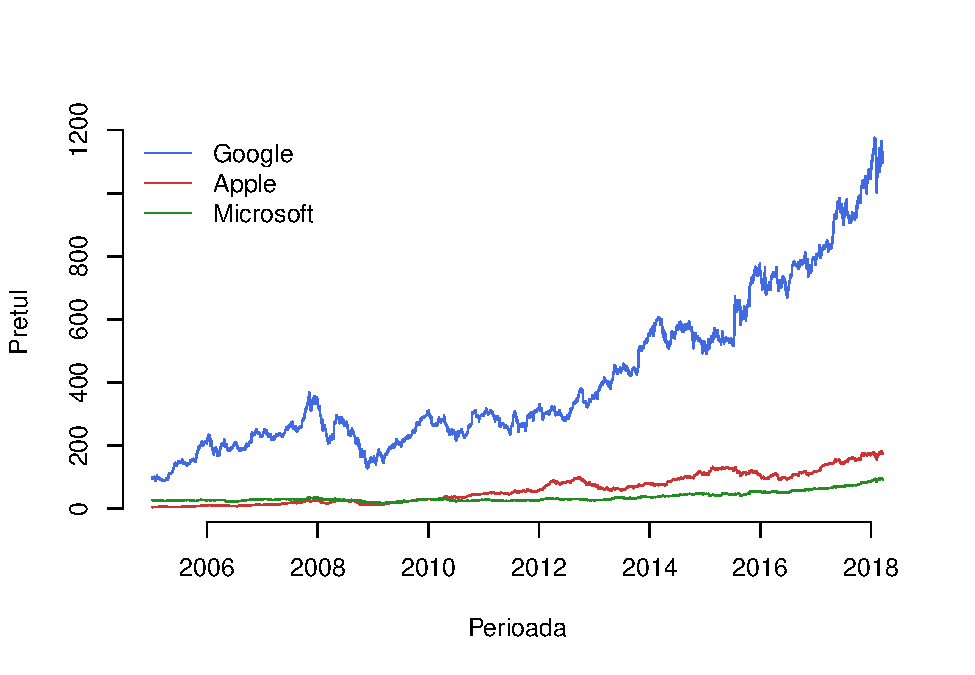
\includegraphics[width=0.8\linewidth]{Lab_3_files/figure-latex/unnamed-chunk-7-1} \end{center}

\section{Rentabilitate (Returns)}\label{rentabilitate-returns}

Scopul unei investiții este acela de a face profit, prin urmare
investitorii sunt interesași în a face investiții care produc venituri
mari relativ la mărimea investiției. Rentabilitatea / Rata de
rentabilitate (returns) măsoară modificarea prețului unui bun exprimat
ca o fracție din prețul inițial.

\subsection{Rentabilitate netă și brută (net and gross
return)}\label{rentabilitate-neta-si-bruta-net-and-gross-return}

Să presupunem că achiziționăm un bun (activ, stock, etc.) la momentul
\(t_0\) cu prețul \(P_{t_0}\) și îl vindem la momentul \(t_1\) cu prețul
\(P_{t_1}\). Dacă între \(t_0\) și \(t_1\) nu avem schimbări de preț
atunci rata de rentabilitate pe perioada \(t_0\) - \(t_1\) este

\[
  R(t_0,t_1) = \frac{P_{t_1} - P_{t_0}}{P_{t_0}}.
\]

Perioada dintre \(t_0\) și \(t_1\) se numește perioada de retenție a
bunului (\emph{holding period}), perioada dintre achiziția și vânzarea
unui bun (activ, etc.), și poate fi măsurată în secunde, minute, ore,
zile, luni, etc. Dacă \(P_t\) este prețul unui activ la momentul \(t\)
(să zicem la sfârșitul lunii \(t\)) și \(P_{t-1}\) este prețul activului
la momentul \(t-1\) atunci rentabilitatea netă (\emph{net return}) în
perioada de la \(t-1\) la \(t\) este

\[
  R_t = \frac{P_{t} - P_{t-1}}{P_{t-1}}
\]

și putem spune că

\[
  \text{venitul } = \text{ investitia initiala } \times \text{ rentabilitatea neta}.
\]

Rentabilitatea brută (\emph{gross return}) este definită prin

\[
  \frac{P_{t}}{P_{t-1}} = 1 + R_t.
\]

Spre exemplu să considerăm o investiție de o lună într-un stock
Microsoft. Să presupunem că achiziționăm stock-ul în luna \(t-1\) cu
prețul \(P_{t-1} = 85\, u.m.\) și îl vindem în luna următoare cu
\(P_{t} = 90\, u.m.\). Atunci rentabilitatea netă și brută pe perioada
de 1 lună sunt: \(R_t = \frac{90-85}{85} = 0.058\) iar \(1+R_t = 1.058\)
ceea ce înseamnă că investiția a condus la o rentabiltate de \(5.8\%\)
sau altfel spus \(1\,u.m.\) investită în stock-ul Microsoft în luna
\(t-1\) a crescut la \(1.058\,u.m.\) în luna \(t\) (creșterea a fost de
\(105.8\%\)).

Să presupunem că vrem să calculăm rentabilitatea zilnică (netă și brută)
a stock-urilor Apple, Google și Microsoft:

\begin{Shaded}
\begin{Highlighting}[]
\CommentTok{# Rentabilitatea zilnica }
\NormalTok{google_ret_s_daily =}\StringTok{ }\NormalTok{google_data}\OperatorTok{$}\NormalTok{Close[}\OperatorTok{-}\DecValTok{1}\NormalTok{] }\OperatorTok{/}\StringTok{ }\NormalTok{google_data}\OperatorTok{$}\NormalTok{Close[}\OperatorTok{-}\KeywordTok{length}\NormalTok{(google_data}\OperatorTok{$}\NormalTok{Close)] }\OperatorTok{-}\StringTok{ }\DecValTok{1} 
\NormalTok{apple_ret_s_daily =}\StringTok{ }\NormalTok{apple_data}\OperatorTok{$}\NormalTok{Close[}\OperatorTok{-}\DecValTok{1}\NormalTok{] }\OperatorTok{/}\StringTok{ }\NormalTok{apple_data}\OperatorTok{$}\NormalTok{Close[}\OperatorTok{-}\KeywordTok{length}\NormalTok{(apple_data}\OperatorTok{$}\NormalTok{Close)] }\OperatorTok{-}\StringTok{ }\DecValTok{1} 
\NormalTok{msft_ret_s_daily =}\StringTok{ }\NormalTok{msft_data}\OperatorTok{$}\NormalTok{Close[}\OperatorTok{-}\DecValTok{1}\NormalTok{] }\OperatorTok{/}\StringTok{ }\NormalTok{msft_data}\OperatorTok{$}\NormalTok{Close[}\OperatorTok{-}\KeywordTok{length}\NormalTok{(msft_data}\OperatorTok{$}\NormalTok{Close)] }\OperatorTok{-}\StringTok{ }\DecValTok{1} 

\KeywordTok{head}\NormalTok{(}\KeywordTok{cbind}\NormalTok{(google_ret_s_daily, apple_ret_s_daily, msft_ret_s_daily))}
\NormalTok{     google_ret_s_daily apple_ret_s_daily msft_ret_s_daily}
\NormalTok{[}\DecValTok{1}\NormalTok{,]       }\OperatorTok{-}\FloatTok{0.040501234}      \FloatTok{0.0102702803}      \FloatTok{0.003739716}
\NormalTok{[}\DecValTok{2}\NormalTok{,]       }\OperatorTok{-}\FloatTok{0.005089951}      \FloatTok{0.0087582105}     \OperatorTok{-}\FloatTok{0.002235432}
\NormalTok{[}\DecValTok{3}\NormalTok{,]       }\OperatorTok{-}\FloatTok{0.025631748}      \FloatTok{0.0007751008}     \OperatorTok{-}\FloatTok{0.001120276}
\NormalTok{[}\DecValTok{4}\NormalTok{,]        }\FloatTok{0.028109237}      \FloatTok{0.0728119332}     \OperatorTok{-}\FloatTok{0.002990654}
\NormalTok{[}\DecValTok{5}\NormalTok{,]        }\FloatTok{0.006241924}     \OperatorTok{-}\FloatTok{0.0041878697}      \FloatTok{0.004874353}
\NormalTok{[}\DecValTok{6}\NormalTok{,]       }\OperatorTok{-}\FloatTok{0.007792465}     \OperatorTok{-}\FloatTok{0.0638049631}     \OperatorTok{-}\FloatTok{0.002611903}
\end{Highlighting}
\end{Shaded}

\begin{center}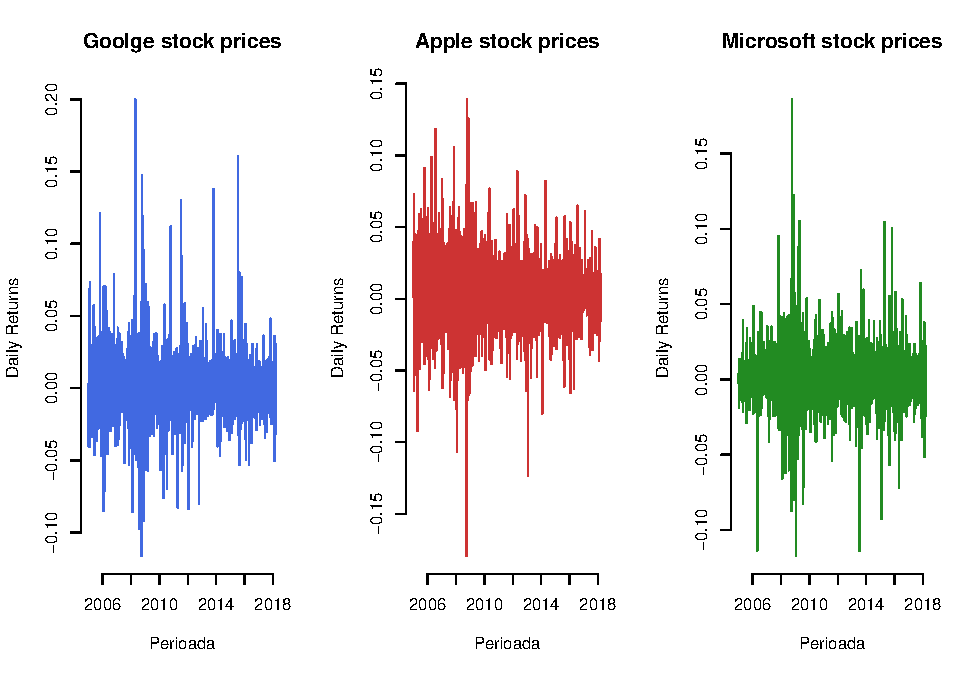
\includegraphics[width=0.8\linewidth]{Lab_3_files/figure-latex/unnamed-chunk-9-1} \end{center}

și rentabilitatea lunară:

\begin{Shaded}
\begin{Highlighting}[]
\CommentTok{# Rentabilitatea lunara}
\NormalTok{returnMonth =}\StringTok{ }\ControlFlowTok{function}\NormalTok{(dat)\{}
\NormalTok{  dat}\OperatorTok{$}\NormalTok{Day =}\StringTok{ }\KeywordTok{as.numeric}\NormalTok{(}\KeywordTok{strftime}\NormalTok{(dat}\OperatorTok{$}\NormalTok{Date, }\StringTok{"%d"}\NormalTok{))}
\NormalTok{  dat}\OperatorTok{$}\NormalTok{Month =}\StringTok{ }\KeywordTok{as.numeric}\NormalTok{(}\KeywordTok{strftime}\NormalTok{(dat}\OperatorTok{$}\NormalTok{Date, }\StringTok{"%m"}\NormalTok{))}
\NormalTok{  dat}\OperatorTok{$}\NormalTok{Year =}\StringTok{ }\KeywordTok{as.numeric}\NormalTok{(}\KeywordTok{strftime}\NormalTok{(dat}\OperatorTok{$}\NormalTok{Date, }\StringTok{"%Y"}\NormalTok{))}
  
\NormalTok{  dat_month_diff =}\StringTok{ }\KeywordTok{diff}\NormalTok{(dat}\OperatorTok{$}\NormalTok{Month)}
\NormalTok{  dat_month =}\StringTok{ }\NormalTok{dat[dat_month_diff }\OperatorTok{>=}\StringTok{ }\DecValTok{1}\NormalTok{, ]}
  
\NormalTok{  month_ret =}\StringTok{ }\NormalTok{dat_month}\OperatorTok{$}\NormalTok{Close[}\OperatorTok{-}\DecValTok{1}\NormalTok{] }\OperatorTok{/}\StringTok{ }\NormalTok{dat_month}\OperatorTok{$}\NormalTok{Close[}\OperatorTok{-}\KeywordTok{length}\NormalTok{(dat_month}\OperatorTok{$}\NormalTok{Close)] }\OperatorTok{-}\StringTok{ }\DecValTok{1} 
  \KeywordTok{return}\NormalTok{(}\KeywordTok{data.frame}\NormalTok{(}\DataTypeTok{date =}\NormalTok{ dat_month}\OperatorTok{$}\NormalTok{Date[}\OperatorTok{-}\DecValTok{1}\NormalTok{], }\DataTypeTok{ret =}\NormalTok{ month_ret))}
\NormalTok{\}}

\NormalTok{google_ret_s_monthly =}\StringTok{ }\KeywordTok{returnMonth}\NormalTok{(google_data)}
\NormalTok{apple_ret_s_monthly =}\StringTok{ }\KeywordTok{returnMonth}\NormalTok{(apple_data)}
\NormalTok{msft_ret_s_monthly =}\StringTok{ }\KeywordTok{returnMonth}\NormalTok{(msft_data)}

\KeywordTok{head}\NormalTok{(}\KeywordTok{cbind}\NormalTok{(google_ret_s_monthly}\OperatorTok{$}\NormalTok{ret, apple_ret_s_monthly}\OperatorTok{$}\NormalTok{ret, }
\NormalTok{           msft_ret_s_monthly}\OperatorTok{$}\NormalTok{ret))}
\NormalTok{            [,}\DecValTok{1}\NormalTok{]        [,}\DecValTok{2}\NormalTok{]        [,}\DecValTok{3}\NormalTok{]}
\NormalTok{[}\DecValTok{1}\NormalTok{,] }\OperatorTok{-}\FloatTok{0.03900416}  \FloatTok{0.16670997} \OperatorTok{-}\FloatTok{0.04261800}
\NormalTok{[}\DecValTok{2}\NormalTok{,] }\OperatorTok{-}\FloatTok{0.03978939} \OperatorTok{-}\FloatTok{0.07111008} \OperatorTok{-}\FloatTok{0.03934817}
\NormalTok{[}\DecValTok{3}\NormalTok{,]  }\FloatTok{0.21876907} \OperatorTok{-}\FloatTok{0.13462914}  \FloatTok{0.04675213}
\NormalTok{[}\DecValTok{4}\NormalTok{,]  }\FloatTok{0.26031817}  \FloatTok{0.10260667}  \FloatTok{0.01976285}
\NormalTok{[}\DecValTok{5}\NormalTok{,]  }\FloatTok{0.06087933} \OperatorTok{-}\FloatTok{0.07419507} \OperatorTok{-}\FloatTok{0.03720927}
\NormalTok{[}\DecValTok{6}\NormalTok{,] }\OperatorTok{-}\FloatTok{0.02172367}  \FloatTok{0.15865239}  \FloatTok{0.03099843}
\end{Highlighting}
\end{Shaded}

\begin{center}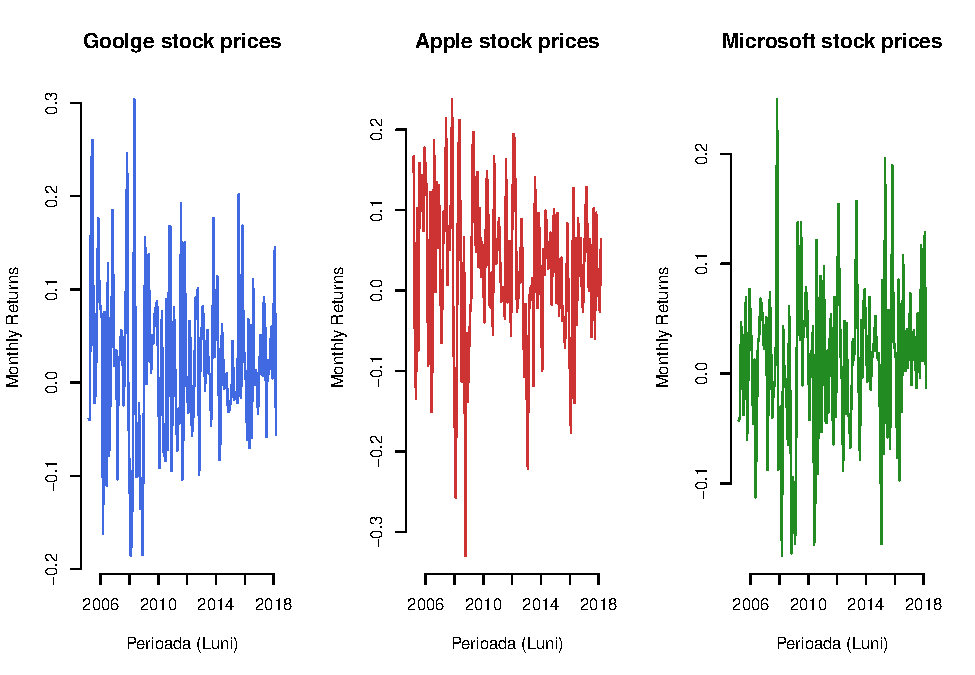
\includegraphics[width=0.8\linewidth]{Lab_3_files/figure-latex/unnamed-chunk-11-1} \end{center}

Rentabilitatea brută pe o \(k\)-perioadă (dacă \(k=2\) și perioada este
o lună atunci avem rentabilitatea brută pentru 2 luni) este dată de
formula

\[
  1+R_{t}(k) = \frac{P_t}{P_{t-k}} = \frac{P_{t}}{P_{t-1}}\frac{P_{t-1}}{P_{t-2}}\cdots \frac{P_{t-k+1}}{P_{t-k}} = \prod_{j=0}^{k-1}(1+R_{t-j}).
\]

\subsection{Rentabilitate compusă / logaritmică (log
returns)}\label{rentabilitate-compusa-logaritmica-log-returns}

Dacă luăm prețurile în scară logaritmică, \(p_t = \log(P_t)\), atunci
definim logaritmul rentabilității - \emph{log returns} (sau
\emph{continuously compounded returns}) prin

\[
  r_t = \log(1+R_t) = p_t-p_{t-1}.
\]

Deoarece, pentru \(x\) suficient de mic putem folosi aproximarea
\(\log(1+x)\approx x\), putem spune că \(r_t\approx R_t\) în special
pentru rentabilități calculate pe perioade scurte de timp
(e.g.~zilnice).

\begin{center}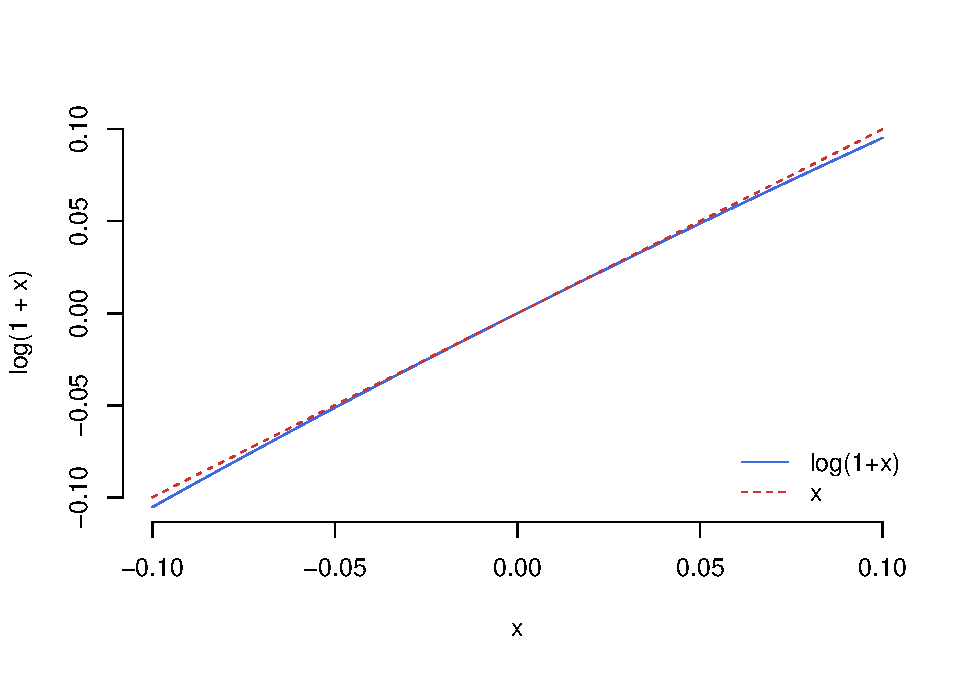
\includegraphics[width=0.8\linewidth]{Lab_3_files/figure-latex/unnamed-chunk-12-1} \end{center}

De asemenea avem că

\[
  r_t(k) = \log(1+R_t(k)) = \log\left(\prod_{j=0}^{k-1}(1+R_{t-j})\right) = \sum_{j = 0}^{k-1}r_{t-j}.
\]

Pentru datele noastre avem

\begin{Shaded}
\begin{Highlighting}[]
\CommentTok{# log returns }
\NormalTok{google_ret_s_monthly}\OperatorTok{$}\NormalTok{cret =}\StringTok{ }\KeywordTok{log}\NormalTok{(}\DecValTok{1}\OperatorTok{+}\NormalTok{google_ret_s_monthly}\OperatorTok{$}\NormalTok{ret)}
\NormalTok{apple_ret_s_monthly}\OperatorTok{$}\NormalTok{cret =}\StringTok{ }\KeywordTok{log}\NormalTok{(}\DecValTok{1}\OperatorTok{+}\NormalTok{apple_ret_s_monthly}\OperatorTok{$}\NormalTok{ret)}
\NormalTok{msft_ret_s_monthly}\OperatorTok{$}\NormalTok{cret =}\StringTok{ }\KeywordTok{log}\NormalTok{(}\DecValTok{1}\OperatorTok{+}\NormalTok{msft_ret_s_monthly}\OperatorTok{$}\NormalTok{ret)}

\CommentTok{# ilustrare grafica}
\KeywordTok{plot}\NormalTok{(google_ret_s_monthly}\OperatorTok{$}\NormalTok{date, google_ret_s_monthly}\OperatorTok{$}\NormalTok{cret,}
     \DataTypeTok{type =} \StringTok{"l"}\NormalTok{, }
     \DataTypeTok{col =} \StringTok{"royalblue"}\NormalTok{,}
     \DataTypeTok{main =} \StringTok{"Goolge - Apple - Microsoft log returns"}\NormalTok{,}
     \DataTypeTok{xlab =} \StringTok{"Perioada (Luni)"}\NormalTok{,}
     \DataTypeTok{ylab =} \StringTok{"Log Returns"}\NormalTok{,}
     \DataTypeTok{bty =} \StringTok{"n"}\NormalTok{)}

\KeywordTok{lines}\NormalTok{(apple_ret_s_monthly}\OperatorTok{$}\NormalTok{date, apple_ret_s_monthly}\OperatorTok{$}\NormalTok{cret,}
      \DataTypeTok{col =} \StringTok{"brown3"}\NormalTok{,}
      \DataTypeTok{lty =} \DecValTok{2}\NormalTok{)}

\KeywordTok{lines}\NormalTok{(msft_ret_s_monthly}\OperatorTok{$}\NormalTok{date, msft_ret_s_monthly}\OperatorTok{$}\NormalTok{cret,}
      \DataTypeTok{col =} \StringTok{"forestgreen"}\NormalTok{,}
      \DataTypeTok{lty =} \DecValTok{3}\NormalTok{)}

\KeywordTok{legend}\NormalTok{(}\StringTok{"bottomright"}\NormalTok{, }
       \DataTypeTok{legend =} \KeywordTok{c}\NormalTok{(}\StringTok{"Google"}\NormalTok{, }\StringTok{"Apple"}\NormalTok{, }\StringTok{"Microsoft"}\NormalTok{), }
       \DataTypeTok{col =} \KeywordTok{c}\NormalTok{(}\StringTok{"royalblue"}\NormalTok{, }\StringTok{"brown3"}\NormalTok{, }\StringTok{"forestgreen"}\NormalTok{), }
       \DataTypeTok{lty =} \KeywordTok{c}\NormalTok{(}\DecValTok{1}\NormalTok{,}\DecValTok{2}\NormalTok{,}\DecValTok{3}\NormalTok{),}
       \DataTypeTok{bty =} \StringTok{"n"}\NormalTok{)}
\end{Highlighting}
\end{Shaded}

\begin{center}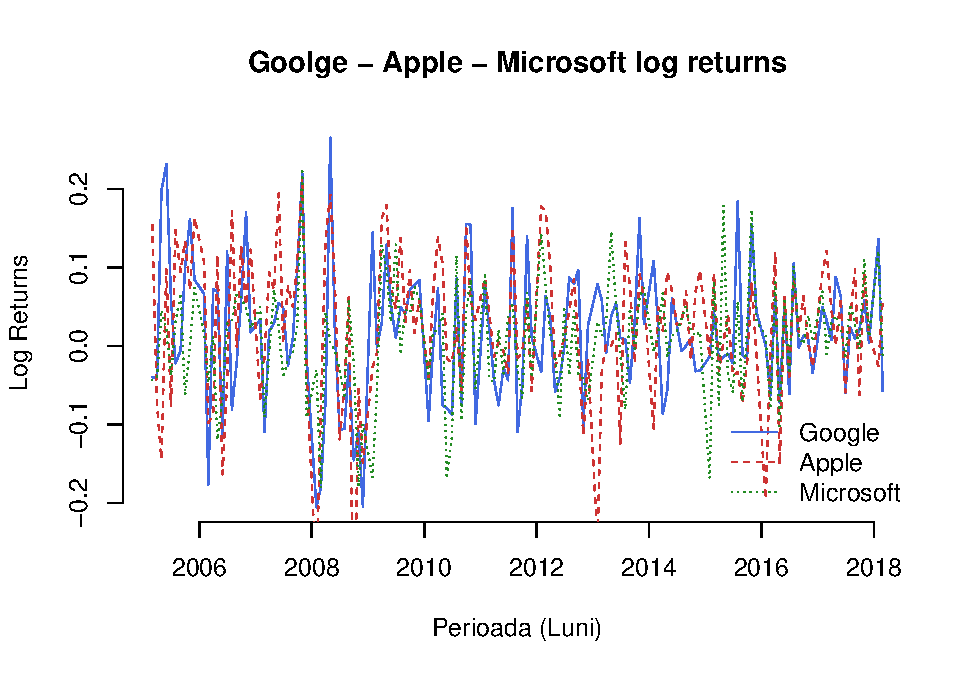
\includegraphics[width=0.8\linewidth]{Lab_3_files/figure-latex/unnamed-chunk-13-1} \end{center}

\subsection{Ajustarea pentru
dividende}\label{ajustarea-pentru-dividende}

Dacă un activ plătește un
\href{https://ro.wikipedia.org/wiki/Dividend}{dividend} \(D_t\) undeva
între momentul de timp \(t-1\) și \(t\) atunci rentabilitatea brută la
momentul \(t\) se calculează după formula

\[
  1+R_t = \frac{P_t+D_t}{P_{t-1}}
\] iar rentabilitatea netă este
\(R_t = \frac{P_t+D_t-P_{t-1}}{P_{t-1}} = \frac{P_t-P_{t-1}}{P_{t-1}} + \frac{D_t}{P_{t-1}}\)
unde \(\frac{P_t-P_{t-1}}{P_{t-1}}\) se numește câștigul de capital
(\emph{capital gain}) iar \(\frac{D_t}{P_{t-1}}\) se numește randamentul
dividendului (\emph{dividend yield}). Avem astfel că

\[
  1+R_{t}(k) = \prod_{j=0}^{k-1}\frac{P_{t-j}+D_{t-j}}{P_{t-j-1}} = \prod_{j=0}^{k-1}(1+R_{t-j})
\]

iar

\[
  r_t(k) = \log(1+R_t(k)) = \sum_{j=0}^{k-1}\log\left(\frac{P_{t-j}+D_{t-j}}{P_{t-j-1}}\right).
\] Pentru a calcula rentabilitățile ajustate vom folosi coloana
\texttt{Adjusted} (care apare doar la datele de pe Yahoo Finance !):

\begin{Shaded}
\begin{Highlighting}[]
\CommentTok{# Rentabilitatea lunara ajustata pentru dividende }
\NormalTok{returnMonthAdjusted =}\StringTok{ }\ControlFlowTok{function}\NormalTok{(dat)\{}
\NormalTok{  dat}\OperatorTok{$}\NormalTok{Day =}\StringTok{ }\KeywordTok{as.numeric}\NormalTok{(}\KeywordTok{strftime}\NormalTok{(dat}\OperatorTok{$}\NormalTok{Date, }\StringTok{"%d"}\NormalTok{))}
\NormalTok{  dat}\OperatorTok{$}\NormalTok{Month =}\StringTok{ }\KeywordTok{as.numeric}\NormalTok{(}\KeywordTok{strftime}\NormalTok{(dat}\OperatorTok{$}\NormalTok{Date, }\StringTok{"%m"}\NormalTok{))}
\NormalTok{  dat}\OperatorTok{$}\NormalTok{Year =}\StringTok{ }\KeywordTok{as.numeric}\NormalTok{(}\KeywordTok{strftime}\NormalTok{(dat}\OperatorTok{$}\NormalTok{Date, }\StringTok{"%Y"}\NormalTok{))}
  
\NormalTok{  dat_month_diff =}\StringTok{ }\KeywordTok{diff}\NormalTok{(dat}\OperatorTok{$}\NormalTok{Month)}
\NormalTok{  dat_month =}\StringTok{ }\NormalTok{dat[dat_month_diff }\OperatorTok{==}\StringTok{ }\DecValTok{1}\NormalTok{, ]}
  
\NormalTok{  month_ret =}\StringTok{ }\NormalTok{dat_month}\OperatorTok{$}\NormalTok{Adjusted[}\OperatorTok{-}\DecValTok{1}\NormalTok{] }\OperatorTok{/}\StringTok{ }\NormalTok{dat_month}\OperatorTok{$}\NormalTok{Adjusted[}\OperatorTok{-}\KeywordTok{length}\NormalTok{(dat_month}\OperatorTok{$}\NormalTok{Adjusted)] }\OperatorTok{-}\StringTok{ }\DecValTok{1} 
  \KeywordTok{return}\NormalTok{(}\KeywordTok{data.frame}\NormalTok{(}\DataTypeTok{date =}\NormalTok{ dat_month}\OperatorTok{$}\NormalTok{Date[}\OperatorTok{-}\DecValTok{1}\NormalTok{], }\DataTypeTok{ret =}\NormalTok{ month_ret))}
\NormalTok{\}}

\NormalTok{google_ret_adj_monthly =}\StringTok{ }\KeywordTok{returnMonthAdjusted}\NormalTok{(google_data)}
\NormalTok{apple_ret_adj_monthly =}\StringTok{ }\KeywordTok{returnMonthAdjusted}\NormalTok{(apple_data)}
\NormalTok{msft_ret_adj_monthly =}\StringTok{ }\KeywordTok{returnMonthAdjusted}\NormalTok{(msft_data)}

\KeywordTok{head}\NormalTok{(}\KeywordTok{cbind}\NormalTok{(google_ret_adj_monthly}\OperatorTok{$}\NormalTok{ret, apple_ret_adj_monthly}\OperatorTok{$}\NormalTok{ret, }
\NormalTok{           msft_ret_adj_monthly}\OperatorTok{$}\NormalTok{ret))}
\NormalTok{            [,}\DecValTok{1}\NormalTok{]        [,}\DecValTok{2}\NormalTok{]        [,}\DecValTok{3}\NormalTok{]}
\NormalTok{[}\DecValTok{1}\NormalTok{,] }\OperatorTok{-}\FloatTok{0.03900416}  \FloatTok{0.16670979} \OperatorTok{-}\FloatTok{0.03966420}
\NormalTok{[}\DecValTok{2}\NormalTok{,] }\OperatorTok{-}\FloatTok{0.03978939} \OperatorTok{-}\FloatTok{0.07110995} \OperatorTok{-}\FloatTok{0.03934825}
\NormalTok{[}\DecValTok{3}\NormalTok{,]  }\FloatTok{0.21876907} \OperatorTok{-}\FloatTok{0.13462939}  \FloatTok{0.04675180}
\NormalTok{[}\DecValTok{4}\NormalTok{,]  }\FloatTok{0.26031817}  \FloatTok{0.10260652}  \FloatTok{0.02299797}
\NormalTok{[}\DecValTok{5}\NormalTok{,]  }\FloatTok{0.06087933} \OperatorTok{-}\FloatTok{0.07419498} \OperatorTok{-}\FloatTok{0.03720931}
\NormalTok{[}\DecValTok{6}\NormalTok{,] }\OperatorTok{-}\FloatTok{0.02172367}  \FloatTok{0.15865307}  \FloatTok{0.03099854}

\CommentTok{# log returns }
\NormalTok{google_ret_adj_monthly}\OperatorTok{$}\NormalTok{cret =}\StringTok{ }\KeywordTok{log}\NormalTok{(}\DecValTok{1}\OperatorTok{+}\NormalTok{google_ret_adj_monthly}\OperatorTok{$}\NormalTok{ret)}
\NormalTok{apple_ret_adj_monthly}\OperatorTok{$}\NormalTok{cret =}\StringTok{ }\KeywordTok{log}\NormalTok{(}\DecValTok{1}\OperatorTok{+}\NormalTok{apple_ret_adj_monthly}\OperatorTok{$}\NormalTok{ret)}
\NormalTok{msft_ret_adj_monthly}\OperatorTok{$}\NormalTok{cret =}\StringTok{ }\KeywordTok{log}\NormalTok{(}\DecValTok{1}\OperatorTok{+}\NormalTok{msft_ret_adj_monthly}\OperatorTok{$}\NormalTok{ret)}
\end{Highlighting}
\end{Shaded}

\begin{center}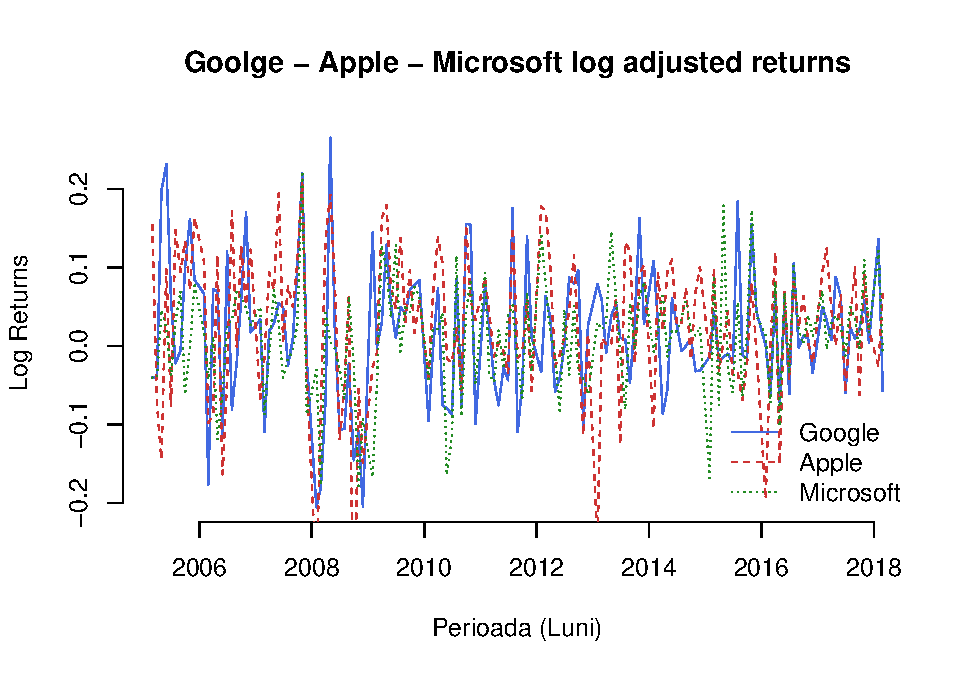
\includegraphics[width=0.8\linewidth]{Lab_3_files/figure-latex/unnamed-chunk-15-1} \end{center}

\subsection{Modelul mersului la întâmplare
geometric}\label{modelul-mersului-la-intamplare-geometric}

Fie \(Z_1, Z_2, \ldots\) un șir de variabile aleatoare independente și
identic repartizate de medie \(\mu\) și dispersie \(\sigma^2\). Fie
\(S_0\) este un punct de pornire și \(S_t\) poziția după \(t\) pași
atunci când am plecat din \(S_0\)

\[
  S_t = S_0 + Z_1 + Z_2 + \cdots + Z_t, \; t\geq 1.
\]

Procesul \(S_0, S_1, \ldots\) se numește mers la întâmplare iar
\(Z_1, Z_2, \ldots\) sunt pașii. Se poate observa că
\(\mathbb{E}[S_t|S_0] = S_0 + \mu t\) iar \(Var(S_t|S_0) = \sigma^2 t\),
\(\mu\) se numește parametru de \emph{drift} și determină direcția de
deplasare iar \(\sigma\) se numește \emph{volatilitate} și determină cât
de mult fluctuează mersul la întâmplare în jurul mediei condiționare.

Am văzut că rentabilitatea pentru o \(k\)-perioadă verifică

\begin{align*}
  1+R_t(k) &= \left(1+R_{t}\right)\left(1+R_{t+1}\right) \cdots \left(1+R_{t-k+1}\right) = e^{r_t}e^{r_{t+1}}\cdots e^{r_{t-k+1}}\\
           &= e^{r_t+r_{t+1}+\cdots+r_{t-k+1}}
\end{align*}

de unde \(r_t(k) = \log(1+R_t(k)) = r_t+r_{t+1}+\cdots+r_{t-k+1}\).

Ipoteza \emph{mersului la întâmplare} presupune că rentabilitățile
compuse (log-return-urile) \(r_t\) sunt variabile aleatoare independente
și identic repartizate. De asemenea avem că

\[
  \frac{P_{t}}{P_{t-k}} = 1+R_t(k) = e^{r_t+r_{t+1}+\cdots+r_{t-k+1}}
\]

ceea ce conduce la \(P_t = P_0e^{r_t+r_{t+1}+\cdots+r_{t-k+1}}\) (mers
la întâmplare exponențial). În cazul în care
\(r_t\sim\mathcal{N}(\mu, \sigma^2)\) atunci \(P_t\) este o variabilă
aleatoare repartizată log-normal iar procesul \(P_0, P_1, \ldots\) se
numește mers la întâmplare geometric.

Să presupunem că vrem să simulăm în R evoluția prețurilor unui stock
atunci când rentabilitățile compuse (log-return-urile) sunt repartizare
normal, deci prețurile descriu un mers la întâmplare geometric. Vom
simula evoluția prețurilor pe parcursul unui an (în medie sunt
\(n = 253\) de zile de tranzacționare pentru un an) și vom presupune că
prețul inițial a fost de \(120\) u.m..

\begin{Shaded}
\begin{Highlighting}[]
\KeywordTok{set.seed}\NormalTok{(}\DecValTok{2018}\NormalTok{)}
\NormalTok{n =}\StringTok{ }\DecValTok{253}

\NormalTok{P0 =}\StringTok{ }\DecValTok{120}
\NormalTok{mu =}\StringTok{ }\FloatTok{0.05}\OperatorTok{/}\NormalTok{n}
\NormalTok{sigma =}\StringTok{ }\FloatTok{0.2}\OperatorTok{/}\KeywordTok{sqrt}\NormalTok{(n)}

\KeywordTok{par}\NormalTok{(}\DataTypeTok{mfrow=}\KeywordTok{c}\NormalTok{(}\DecValTok{2}\NormalTok{,}\DecValTok{2}\NormalTok{), }\DataTypeTok{bty =} \StringTok{"n"}\NormalTok{)}
\ControlFlowTok{for}\NormalTok{ (i }\ControlFlowTok{in} \DecValTok{1}\OperatorTok{:}\DecValTok{4}\NormalTok{)}
\NormalTok{\{}
\NormalTok{  logr =}\StringTok{ }\KeywordTok{rnorm}\NormalTok{(n, mu, sigma)}
\NormalTok{  price =}\StringTok{ }\KeywordTok{c}\NormalTok{(P0, P0}\OperatorTok{*}\KeywordTok{exp}\NormalTok{(}\KeywordTok{cumsum}\NormalTok{(logr)))}
  
  \KeywordTok{plot}\NormalTok{(price, }\DataTypeTok{type=}\StringTok{"l"}\NormalTok{,}
       \DataTypeTok{xlab =} \StringTok{"Index zile"}\NormalTok{,}
       \DataTypeTok{ylab =} \StringTok{"Pret"}\NormalTok{, }
       \DataTypeTok{col =} \StringTok{"forestgreen"}\NormalTok{)}
\NormalTok{\}}
\end{Highlighting}
\end{Shaded}

\begin{center}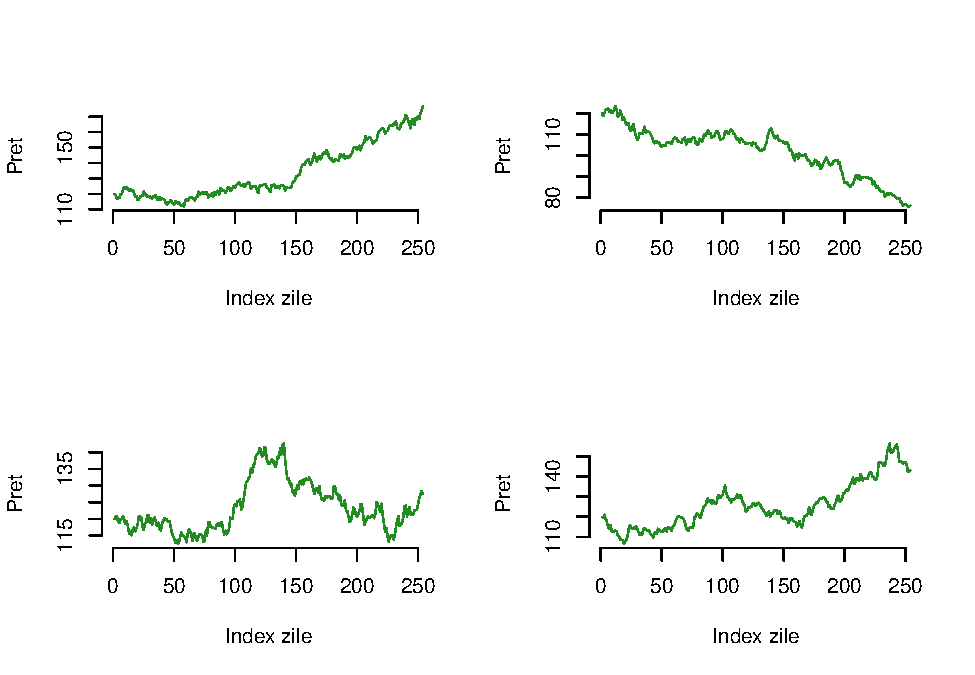
\includegraphics{Lab_3_files/figure-latex/unnamed-chunk-16-1} \end{center}

\begin{Shaded}
\begin{Highlighting}[]
\CommentTok{# Simularea unui proces gausian}

\KeywordTok{library}\NormalTok{(MASS)}
 
\NormalTok{gaussprocess <-}\StringTok{ }\ControlFlowTok{function}\NormalTok{(}\DataTypeTok{from =} \DecValTok{0}\NormalTok{, }\DataTypeTok{to =} \DecValTok{1}\NormalTok{, }
                         \DataTypeTok{K =} \ControlFlowTok{function}\NormalTok{(s, t) \{}\KeywordTok{min}\NormalTok{(s, t)\},}
                         \DataTypeTok{start =} \OtherTok{NULL}\NormalTok{, }\DataTypeTok{m =} \DecValTok{1000}\NormalTok{) \{}
  \CommentTok{# Simuleaza un proces Gausian cu functia nucleu K}
  \CommentTok{#}
  \CommentTok{# args:}
  \CommentTok{#   from: Punct de plecare}
  \CommentTok{#   to: Punct final }
  \CommentTok{#   K: functie nucleu; default proces Wiener}
  \CommentTok{#   start: pozitie de start}
  \CommentTok{#   m: nr de puncte simulate }
  \CommentTok{#}
  \CommentTok{# return:}
  \CommentTok{#   un data.frame in care primul arg este timpul iar }
  \CommentTok{#   al doilea este xt procesul }
   
\NormalTok{  t =}\StringTok{ }\KeywordTok{seq}\NormalTok{(}\DataTypeTok{from =}\NormalTok{ from, }\DataTypeTok{to =}\NormalTok{ to, }\DataTypeTok{length.out =}\NormalTok{ m)}
  
\NormalTok{  Sigma =}\StringTok{ }\KeywordTok{sapply}\NormalTok{(t, }\ControlFlowTok{function}\NormalTok{(s1) \{}
    \KeywordTok{sapply}\NormalTok{(t, }\ControlFlowTok{function}\NormalTok{(s2) \{}
      \KeywordTok{K}\NormalTok{(s1, s2)}
\NormalTok{    \})}
\NormalTok{  \})}
   
\NormalTok{  path =}\StringTok{ }\KeywordTok{mvrnorm}\NormalTok{(}\DataTypeTok{mu =} \KeywordTok{rep}\NormalTok{(}\DecValTok{0}\NormalTok{, }\DataTypeTok{times =}\NormalTok{ m), }\DataTypeTok{Sigma =}\NormalTok{ Sigma)}
  
  \ControlFlowTok{if}\NormalTok{ (}\OperatorTok{!}\KeywordTok{is.null}\NormalTok{(start)) \{}
\NormalTok{    path <-}\StringTok{ }\NormalTok{path }\OperatorTok{-}\StringTok{ }\NormalTok{path[}\DecValTok{1}\NormalTok{] }\OperatorTok{+}\StringTok{ }\NormalTok{start  }
\NormalTok{  \}}
   
  \KeywordTok{return}\NormalTok{(}\KeywordTok{data.frame}\NormalTok{(}\StringTok{"t"}\NormalTok{ =}\StringTok{ }\NormalTok{t, }\StringTok{"xt"}\NormalTok{ =}\StringTok{ }\NormalTok{path))}
\NormalTok{\}}
\end{Highlighting}
\end{Shaded}

\section{Măsuri de centralitate: media, mediana și
modul}\label{masuri-de-centralitate-media-mediana-si-modul}

\subsection{Media}\label{media}

Media eșantionului este considerată ca fiind punctul central care
balansează colecția de observații și se calculează după formula

\[
  \bar{X}_n = \frac{X_1+X_2+\cdots +X_n}{n}
\]

De exemplu prețul mediu la închidere pentru stoc-urile Apple, Microsoft
și respectiv Google sunt

\begin{Shaded}
\begin{Highlighting}[]
\NormalTok{x.bar.apple =}\StringTok{ }\KeywordTok{mean}\NormalTok{(apple_data}\OperatorTok{$}\NormalTok{Close)}
\NormalTok{x.bar.msft =}\StringTok{ }\KeywordTok{mean}\NormalTok{(msft_data}\OperatorTok{$}\NormalTok{Close)}
\NormalTok{x.bar.google =}\StringTok{ }\KeywordTok{mean}\NormalTok{(google_data}\OperatorTok{$}\NormalTok{Close)}

\NormalTok{x.bar.apple}
\NormalTok{[}\DecValTok{1}\NormalTok{] }\FloatTok{62.01289}
\NormalTok{x.bar.msft}
\NormalTok{[}\DecValTok{1}\NormalTok{] }\FloatTok{36.59903}
\NormalTok{x.bar.google}
\NormalTok{[}\DecValTok{1}\NormalTok{] }\FloatTok{410.8778}
\end{Highlighting}
\end{Shaded}

iar prețul mediu la închidere din anul 2017 pentru cele 3 stoc-uri a
fost

\begin{Shaded}
\begin{Highlighting}[]
\KeywordTok{mean}\NormalTok{(apple_data}\OperatorTok{$}\NormalTok{Close[}\KeywordTok{strftime}\NormalTok{(apple_data}\OperatorTok{$}\NormalTok{Date, }\StringTok{"%Y"}\NormalTok{) }\OperatorTok{==}\StringTok{ "2017"}\NormalTok{])}
\NormalTok{[}\DecValTok{1}\NormalTok{] }\FloatTok{150.5511}
\KeywordTok{mean}\NormalTok{(msft_data}\OperatorTok{$}\NormalTok{Close[}\KeywordTok{strftime}\NormalTok{(msft_data}\OperatorTok{$}\NormalTok{Date, }\StringTok{"%Y"}\NormalTok{) }\OperatorTok{==}\StringTok{ "2017"}\NormalTok{])}
\NormalTok{[}\DecValTok{1}\NormalTok{] }\FloatTok{71.98402}
\KeywordTok{mean}\NormalTok{(google_data}\OperatorTok{$}\NormalTok{Close[}\KeywordTok{strftime}\NormalTok{(google_data}\OperatorTok{$}\NormalTok{Date, }\StringTok{"%Y"}\NormalTok{) }\OperatorTok{==}\StringTok{ "2017"}\NormalTok{])}
\NormalTok{[}\DecValTok{1}\NormalTok{] }\FloatTok{921.7808}
\end{Highlighting}
\end{Shaded}

\subsection{Mediana}\label{mediana}

Mediana este acea valoare pentru care aproximativ \(50\%\) dintre
observații sunt mai mici și \(50\%\) dintre observații sunt mai mari, se
mai numește și magnitudinea de mijloc a obsevațiilor. Mediana (empirică)
se găsește cu ajutorul formulei

\[
  M_n = \left\{\begin{array}{ll}
      X_{\left(\frac{n+1}{2}\right)}, & \text{$n$ este impar}\\
      \frac{X_{\left(\frac{n}{2}\right)} + X_{\left(\frac{n}{2}+1\right)}}{2}, & \text{$n$ este par}
  \end{array}\right.
\]

unde \(X_{(i)}\) este a \(i\)-a cea mai mică observație a eșantionului
\(X_1, X_2, \ldots, X_n\) (statistica de ordine de rang \(i\)). A se
vedea secțiunea \protect\hyperlink{sec:cuantile}{Cuantile teoretice}.

În R mediana se calculează cu ajutorul funcției \texttt{median()}.
Prețul median de închidere pentru cele 3 stoc-uri a fost

\begin{Shaded}
\begin{Highlighting}[]
\NormalTok{M.bar.apple =}\StringTok{ }\KeywordTok{median}\NormalTok{(apple_data}\OperatorTok{$}\NormalTok{Close)}
\NormalTok{M.bar.msft =}\StringTok{ }\KeywordTok{median}\NormalTok{(msft_data}\OperatorTok{$}\NormalTok{Close)}
\NormalTok{M.bar.google =}\StringTok{ }\KeywordTok{median}\NormalTok{(google_data}\OperatorTok{$}\NormalTok{Close)}
\end{Highlighting}
\end{Shaded}

iar pentru anii \(2008-2009\) a fost

\begin{Shaded}
\begin{Highlighting}[]
\KeywordTok{median}\NormalTok{(apple_data}\OperatorTok{$}\NormalTok{Close[}\KeywordTok{strftime}\NormalTok{(apple_data}\OperatorTok{$}\NormalTok{Date, }\StringTok{"%Y"}\NormalTok{) }\OperatorTok\StringTok{ }\KeywordTok{c}\NormalTok{(}\StringTok{"2008"}\NormalTok{, }\StringTok{"2009"}\NormalTok{)])}
\NormalTok{[}\DecValTok{1}\NormalTok{] }\FloatTok{20.53429}
\KeywordTok{median}\NormalTok{(msft_data}\OperatorTok{$}\NormalTok{Close[}\KeywordTok{strftime}\NormalTok{(msft_data}\OperatorTok{$}\NormalTok{Date, }\StringTok{"%Y"}\NormalTok{)  }\OperatorTok\StringTok{ }\KeywordTok{c}\NormalTok{(}\StringTok{"2008"}\NormalTok{, }\StringTok{"2009"}\NormalTok{)])}
\NormalTok{[}\DecValTok{1}\NormalTok{] }\FloatTok{25.3}
\KeywordTok{median}\NormalTok{(google_data}\OperatorTok{$}\NormalTok{Close[}\KeywordTok{strftime}\NormalTok{(google_data}\OperatorTok{$}\NormalTok{Date, }\StringTok{"%Y"}\NormalTok{) }\OperatorTok\StringTok{ }\KeywordTok{c}\NormalTok{(}\StringTok{"2008"}\NormalTok{, }\StringTok{"2009"}\NormalTok{)])}
\NormalTok{[}\DecValTok{1}\NormalTok{] }\FloatTok{224.1124}
\end{Highlighting}
\end{Shaded}

\subsection{Modul}\label{modul}

Modul este valoarea cea mai frecventă din setul de date. Un set de date
poate să nu aibă mod (de exemplu dacă frecvența de apariție a
observațiilor este 1 - toate apar o singură dată), să aibă un mod, două
moduri (set bimodal) sau mai multe.

Care au fost lunile cu cele mai multe tranzacții pentru cele 3 stoc-uri:

\begin{Shaded}
\begin{Highlighting}[]
\CommentTok{# Apple}
\NormalTok{xtab.apple =}\StringTok{ }\KeywordTok{table}\NormalTok{(}\KeywordTok{strftime}\NormalTok{(apple_data}\OperatorTok{$}\NormalTok{Date, }\StringTok{"%b"}\NormalTok{))}
\NormalTok{xtab.apple[xtab.apple }\OperatorTok{==}\StringTok{ }\KeywordTok{max}\NormalTok{(xtab.apple)]}
\NormalTok{Mar }
\DecValTok{299} 

\CommentTok{# Microsoft}
\NormalTok{xtab.msft =}\StringTok{ }\KeywordTok{table}\NormalTok{(}\KeywordTok{strftime}\NormalTok{(msft_data}\OperatorTok{$}\NormalTok{Date, }\StringTok{"%b"}\NormalTok{))}
\NormalTok{xtab.msft[xtab.msft }\OperatorTok{==}\StringTok{ }\KeywordTok{max}\NormalTok{(xtab.msft)]}
\NormalTok{Mar }
\DecValTok{299} 

\CommentTok{# Google}
\NormalTok{xtab.google =}\StringTok{ }\KeywordTok{table}\NormalTok{(}\KeywordTok{strftime}\NormalTok{(google_data}\OperatorTok{$}\NormalTok{Date, }\StringTok{"%b"}\NormalTok{))}
\NormalTok{xtab.google[xtab.google }\OperatorTok{==}\StringTok{ }\KeywordTok{max}\NormalTok{(xtab.google)]}
\NormalTok{Mar }
\DecValTok{299} 
\end{Highlighting}
\end{Shaded}

\subsection{Valoarea minimă (Min), valoarea maximă (Max) și intervalul
de valori
(Range)}\label{valoarea-minima-min-valoarea-maxima-max-si-intervalul-de-valori-range}

Pentru a determina valoarea minimă și valoarea maximă a setului de date
putem folosi funcțiile predefinite \texttt{min} și \texttt{max}. De
asemenea pentru a vedea care este intervalul de valori pe care o
variabilă de interes este definită putem aplica funcția \texttt{range}.

De exemplu pentru stoc-ul Apple avem

\begin{Shaded}
\begin{Highlighting}[]
\KeywordTok{min}\NormalTok{(apple_data}\OperatorTok{$}\NormalTok{Close)}
\NormalTok{[}\DecValTok{1}\NormalTok{] }\FloatTok{4.520714}
\KeywordTok{max}\NormalTok{(apple_data}\OperatorTok{$}\NormalTok{Close)}
\NormalTok{[}\DecValTok{1}\NormalTok{] }\FloatTok{181.72}
\KeywordTok{range}\NormalTok{(apple_data}\OperatorTok{$}\NormalTok{Close)}
\NormalTok{[}\DecValTok{1}\NormalTok{]   }\FloatTok{4.520714} \FloatTok{181.720001}
\end{Highlighting}
\end{Shaded}

\hypertarget{sec:cuantile}{\section{Cuantile teoretice și
empirice}\label{sec:cuantile}}

Reamintim că dată fiind o funcție de repartiție \(F\), funcția
\emph{cuantilă} (inversa generalizată) asociată lui \(F\),
\(F^{-1}:(0,1)\to\mathbb{R}\) este definită prin

\[
  F^{-1}(u) = \inf\{x\in\mathbb{R}\,|\,F(x)\geq u\}, \quad \forall u\in(0,1)
\]

unde folosim convențiile \(\inf\mathbb{R} = -\infty\) și
\(\inf\emptyset = +\infty\).

\begin{rmdinsight}
Funcția cuantilă \(F^{-1}\) verifică următoarele proprietăți:

\begin{enumerate}
\def\labelenumi{\arabic{enumi})}
\tightlist
\item
  Valoarea în \(0\): \(F^{-1}(0) = -\infty\)
\item
  Monotonie: \(F^{-1}\) este crescătoare
\item
  Continuitate: \(F^{-1}\) este continuă la stânga
\item
  Echivalență: pentru \(\forall u\in[0,1]\) avem
  \(F(x)\geq u \iff x\geq F^{-1}(u)\)
\item
  Inversabilitate: \(\forall u\in[0,1]\) avem
  \((F\circ F^{-1})(u)\geq u\). În plus

  \begin{enumerate}
  \def\labelenumii{\alph{enumii})}
  \tightlist
  \item
    dacă \(F\) este continuă atunci \(F\circ F^{-1} = Id\) dar dacă nu
    este injectivă atunci există \(x_0\) așa încât
    \((F^{-1}\circ F)(x_0)<x_0\)
  \item
    dacă \(F\) este injectivă atunci \(F^{-1}\circ F = Id\) dar dacă nu
    este continuă atunci există \(u_0\) astfel că
    \((F\circ F^{-1})(u_0)>u_0\)
  \end{enumerate}
\end{enumerate}
\end{rmdinsight}

Pentru a exemplifica punctul 5a, putem considera variabila aleatoare
\(X\sim\mathcal{U}[0,1]\) a cărei funcție de repartiție \(F\) este
continuă dar nu injectivă și în plus
\((F^{-1}\circ F)(2) = F^{-1}(1) = 1 < 2\). Pentru punctul 5b să
considerăm variabilele aleatoare \(Y\sim\mathcal{N}(0,1)\) și
\(B\sim\mathcal{B}(0.5)\) independente și să definim \(X = BY\). Atunci
funcția de repartiție a lui \(X\) verifică \(F(0-) = \frac{1}{4}\) și
\(F(0) = \frac{3}{4}\), este injectivă dar nu și continuă în \(0\) și în
plus avem \((F\circ F^{-1})(1/2) = F(0) = \frac{3}{4}>\frac{1}{2}\).

Se numește \emph{cuantilă} de ordin \(p\in(0,1)\) (sau \(p\)-cuantilă)
asociată lui \(F\) valoarea

\[
  x_p = F^{-1}(p) = \inf\{x\in\mathbb{R}\,|\,F(x)\geq p\}.
\]

Cuantila de ordin \(0.5\), \(x_{\frac{1}{2}}\) se numește mediana lui
\(F\) și se notează cu \(M\)\footnote{Se poate arăta că mediana unei
  v.a. \(X\), cu \(\mathbb{E}[X^2]<\infty\), verifică
  \(x_{\frac{1}{2}} = \arg\min_{t\in\mathbb{R}}\mathbb{E}[|X-t|]\).} sau
\(Q_2\), iar cuantilele de ordin \(\frac{1}{4}\) și respectiv
\(\frac{3}{4}\) se numesc prima și respectiv a treia cuartilă și se
notează cu \(Q_1\) și respectiv \(Q_3\).

Pentru a calcula cuantilele teoretice în R vom folosi funcțiile de tipul
\texttt{qnume\_partiție} unde \texttt{nume\_repartiție} este abrevierea
numelui repartiției \(F\) (e.g. \texttt{unif} pentru uniformă,
\texttt{norm} pentru normală, etc.):

\begin{Shaded}
\begin{Highlighting}[]
\CommentTok{# din repartitia normala}
\KeywordTok{qnorm}\NormalTok{(}\KeywordTok{c}\NormalTok{(}\FloatTok{0.1}\NormalTok{, }\FloatTok{0.25}\NormalTok{, }\FloatTok{0.5}\NormalTok{, }\FloatTok{0.75}\NormalTok{))}
\NormalTok{[}\DecValTok{1}\NormalTok{] }\OperatorTok{-}\FloatTok{1.2815516} \OperatorTok{-}\FloatTok{0.6744898}  \FloatTok{0.0000000}  \FloatTok{0.6744898}

\CommentTok{# din repartitia student cu 5 grade de libertate}
\KeywordTok{qt}\NormalTok{(}\KeywordTok{c}\NormalTok{(}\FloatTok{0.1}\NormalTok{, }\FloatTok{0.25}\NormalTok{, }\FloatTok{0.5}\NormalTok{, }\FloatTok{0.75}\NormalTok{), }\DataTypeTok{df =} \DecValTok{5}\NormalTok{)}
\NormalTok{[}\DecValTok{1}\NormalTok{] }\OperatorTok{-}\FloatTok{1.4758840} \OperatorTok{-}\FloatTok{0.7266868}  \FloatTok{0.0000000}  \FloatTok{0.7266868}
\end{Highlighting}
\end{Shaded}

Fie acum \(X_1,X_2,\ldots,X_n\) un eșantion de talie \(n\) dintr-o
populație a cărei funcție de repartiție este \(F\) și fie \(\hat{F}_n\)
funcția de repartiție empirică asociată. Reamintim că funcția de
repartiție empirică este definită, pentru toate valorile
\(x\in\mathbb{R}\), prin

\[
  \hat{F}_n(x) = \frac{1}{n}\sum_{i = 1}^{n}\mathbf{1}_{(-\infty, x]}(X_i) = \frac{1}{n}\sum_{i = 1}^{n}\mathbf{1}_{(-\infty, x]}(X_{(i)})
\]

unde \(X_{(1)}, X_{(2)}, \ldots, X_{(n)}\) reprezintă statisticile de
ordine. Observăm că, notând \(X_{(n+1)} = +\infty\), avem

\[
  \hat{F}_n(x) = \sum_{i = 1}^{n}\frac{i}{n}\mathbf{1}_{\left[X_{(i)}, X_{(i+1)}\right)}(x).
\]

Pentru \(p\in(0,1)\) definim cuantila empirică de ordin \(p\) și o notăm
\(\hat{x}_p = \hat{x}_p(n)\) valoarea

\[
  \hat{x}_p = \hat{F}_n^{-1}(p) = \inf\{x\in\mathbb{R}\,|\,\hat{F}_n(x)\geq p\}.
\]

Folosind convenția \(X_{(0)}=-\infty\), cunatila empirică de ordin \(p\)
coincide cu una dintre statisticile de ordine:

\[
  \hat{x}_p = X_{(i)} \iff np\leq i< np+1 \iff \hat{x}_p = X_{(\lceil np \rceil)},
\]

unde \(\lceil x \rceil\) reprezintă cea mai mică valoare întreagă mai
mare sau egală cu \(x\).

Pentru calculul cuantilelor empirice vom folosi funcția
\texttt{quantile()}. Articolul (Hyndman and Fan 1996) prezintă și
compară o serie de algoritmi folosiți în soft-urile de profil pentru
calcularea cuantilelor empirice. De exemplu pentru a calcula cuantilele
de ordin 0.25, 0.5 și respectiv 0.75 a prețurilor la închidere a celor
trei stoc-uri avem

\begin{Shaded}
\begin{Highlighting}[]
\KeywordTok{quantile}\NormalTok{(apple_data}\OperatorTok{$}\NormalTok{Close, }\DataTypeTok{prob=}\KeywordTok{c}\NormalTok{(}\FloatTok{0.25}\NormalTok{, }\FloatTok{0.5}\NormalTok{, }\FloatTok{0.75}\NormalTok{))}
     \DecValTok{25}\OperatorTok\StringTok{      }\DecValTok{75}\NormalTok{% }
\FloatTok{18.51357} \FloatTok{53.43286} \FloatTok{98.14250} 
\KeywordTok{quantile}\NormalTok{(msft_data}\OperatorTok{$}\NormalTok{Close, }\DataTypeTok{prob=}\KeywordTok{c}\NormalTok{(}\FloatTok{0.25}\NormalTok{, }\FloatTok{0.5}\NormalTok{, }\FloatTok{0.75}\NormalTok{))}
    \DecValTok{25}\OperatorTok\StringTok{     }\DecValTok{75}\NormalTok{% }
\FloatTok{26.2725} \FloatTok{29.5600} \FloatTok{43.9375} 
\KeywordTok{quantile}\NormalTok{(google_data}\OperatorTok{$}\NormalTok{Close, }\DataTypeTok{prob=}\KeywordTok{c}\NormalTok{(}\FloatTok{0.25}\NormalTok{, }\FloatTok{0.5}\NormalTok{, }\FloatTok{0.75}\NormalTok{))}
     \DecValTok{25}\OperatorTok\StringTok{      }\DecValTok{75}\NormalTok{% }
\FloatTok{233.6727} \FloatTok{301.0867} \FloatTok{555.7454} 
\end{Highlighting}
\end{Shaded}

Aplicând funcția \texttt{fivenum()} (five number summary) variabilei
\texttt{x} obținem cuantilele de ordin 0 (valoarea minimă), 0.25, 0.5
(mediana), 0.75 și respectiv 1 (valoarea maximă) pentru \texttt{x}.

\begin{Shaded}
\begin{Highlighting}[]
\KeywordTok{fivenum}\NormalTok{(apple_data}\OperatorTok{$}\NormalTok{Close)}
\NormalTok{[}\DecValTok{1}\NormalTok{]   }\FloatTok{4.520714}  \FloatTok{18.510000}  \FloatTok{53.432857}  \FloatTok{98.150002} \FloatTok{181.720001}
\end{Highlighting}
\end{Shaded}

O funcție similară care înclude și media observațiilor este funcția
\texttt{summary()}

\begin{Shaded}
\begin{Highlighting}[]
\KeywordTok{summary}\NormalTok{(apple_data}\OperatorTok{$}\NormalTok{Close)}
\NormalTok{   Min. 1st Qu.  Median    Mean 3rd Qu.    Max. }
  \FloatTok{4.521}  \FloatTok{18.514}  \FloatTok{53.433}  \FloatTok{62.013}  \FloatTok{98.142} \FloatTok{181.720} 
\KeywordTok{summary}\NormalTok{(msft_data}\OperatorTok{$}\NormalTok{Close)}
\NormalTok{   Min. 1st Qu.  Median    Mean 3rd Qu.    Max. }
  \FloatTok{15.15}   \FloatTok{26.27}   \FloatTok{29.56}   \FloatTok{36.60}   \FloatTok{43.94}   \FloatTok{96.77} 
\KeywordTok{summary}\NormalTok{(google_data}\OperatorTok{$}\NormalTok{Close)}
\NormalTok{   Min. 1st Qu.  Median    Mean 3rd Qu.    Max. }
  \FloatTok{86.93}  \FloatTok{233.67}  \FloatTok{301.09}  \FloatTok{410.88}  \FloatTok{555.75} \FloatTok{1175.84} 
\end{Highlighting}
\end{Shaded}

\section{Măsuri de variabilitate}\label{masuri-de-variabilitate}

Măsurile de centralitate descrise anterior (media, mediana și modul)
oferă o indicație asupra locației în care sunt centrate datele dar nu
descriu și care este gradul de împrăștiere a acestora. De exemplu
următoarele seturi de date au acceași medie dar gradul de împrăștiere în
raport cu aceasta este diferit.

\begin{Shaded}
\begin{Highlighting}[]
\NormalTok{x =}\StringTok{ }\KeywordTok{c}\NormalTok{(}\FloatTok{4.4}\NormalTok{, }\FloatTok{4.8}\NormalTok{, }\FloatTok{6.1}\NormalTok{, }\FloatTok{5.1}\NormalTok{, }\FloatTok{5.1}\NormalTok{, }\FloatTok{6.2}\NormalTok{, }\FloatTok{5.5}\NormalTok{, }\FloatTok{4.7}\NormalTok{, }\FloatTok{4.3}\NormalTok{, }
      \FloatTok{4.6}\NormalTok{, }\FloatTok{6.2}\NormalTok{, }\FloatTok{5.4}\NormalTok{, }\FloatTok{5.4}\NormalTok{, }\FloatTok{5.1}\NormalTok{, }\FloatTok{4.4}\NormalTok{)}
\KeywordTok{mean}\NormalTok{(x)}
\NormalTok{[}\DecValTok{1}\NormalTok{] }\FloatTok{5.153333}

\NormalTok{y =}\StringTok{ }\KeywordTok{c}\NormalTok{(}\FloatTok{6.8}\NormalTok{, }\FloatTok{5.8}\NormalTok{, }\FloatTok{3.45}\NormalTok{, }\FloatTok{5.85}\NormalTok{, }\FloatTok{4.7}\NormalTok{, }\FloatTok{5.4}\NormalTok{, }\FloatTok{4.8}\NormalTok{, }\FloatTok{4.0}\NormalTok{, }\FloatTok{4.3}\NormalTok{,}
      \FloatTok{4.6}\NormalTok{, }\FloatTok{3.75}\NormalTok{, }\FloatTok{5.8}\NormalTok{, }\FloatTok{7.25}\NormalTok{, }\FloatTok{4.3}\NormalTok{, }\FloatTok{6.5}\NormalTok{)}
\KeywordTok{mean}\NormalTok{(y)}
\NormalTok{[}\DecValTok{1}\NormalTok{] }\FloatTok{5.153333}
\end{Highlighting}
\end{Shaded}

\begin{center}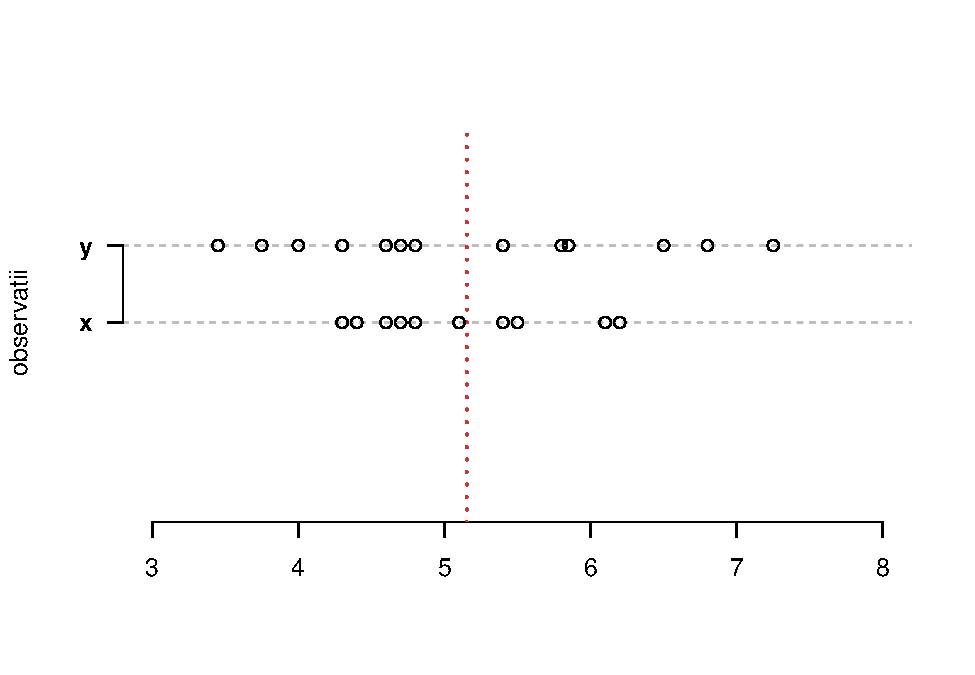
\includegraphics[width=0.8\linewidth]{Lab_3_files/figure-latex/unnamed-chunk-30-1} \end{center}

\subsection{Varianța și abaterea
standard}\label{varianta-si-abaterea-standard}

Varianța eșantionului se calculează cu ajutorul formulei

\[
  S_n^2 = \frac{1}{n-1}\sum_{i=1}^{n}\left(X_i - \bar{X}_n\right)^2
\]

iar abaterea standard a eșantionului este \(s_d = \sqrt{S_n^2}\)
(măsurată în aceleași unități de măsură ca și datele inițiale).

\begin{Shaded}
\begin{Highlighting}[]
\CommentTok{# varianta }
\KeywordTok{var}\NormalTok{(apple_data}\OperatorTok{$}\NormalTok{Close[}\KeywordTok{strftime}\NormalTok{(apple_data}\OperatorTok{$}\NormalTok{Date, }\StringTok{"%Y"}\NormalTok{) }\OperatorTok\StringTok{ }\KeywordTok{c}\NormalTok{(}\StringTok{"2008"}\NormalTok{, }\StringTok{"2009"}\NormalTok{)])}
\NormalTok{[}\DecValTok{1}\NormalTok{] }\FloatTok{27.83872}
\KeywordTok{var}\NormalTok{(msft_data}\OperatorTok{$}\NormalTok{Close[}\KeywordTok{strftime}\NormalTok{(msft_data}\OperatorTok{$}\NormalTok{Date, }\StringTok{"%Y"}\NormalTok{) }\OperatorTok\StringTok{ }\KeywordTok{c}\NormalTok{(}\StringTok{"2008"}\NormalTok{, }\StringTok{"2009"}\NormalTok{)])}
\NormalTok{[}\DecValTok{1}\NormalTok{] }\FloatTok{19.75297}
\KeywordTok{var}\NormalTok{(google_data}\OperatorTok{$}\NormalTok{Close[}\KeywordTok{strftime}\NormalTok{(goole_data}\OperatorTok{$}\NormalTok{Date, }\StringTok{"%Y"}\NormalTok{) }\OperatorTok\StringTok{ }\KeywordTok{c}\NormalTok{(}\StringTok{"2008"}\NormalTok{, }\StringTok{"2009"}\NormalTok{)])}
\NormalTok{Error }\ControlFlowTok{in} \KeywordTok{as.POSIXlt}\NormalTok{(x, }\DataTypeTok{tz =}\NormalTok{ tz)}\OperatorTok{:}\StringTok{ }\NormalTok{object }\StringTok{'goole_data'}\NormalTok{ not found}

\CommentTok{# abaterea standard}
\KeywordTok{sd}\NormalTok{(apple_data}\OperatorTok{$}\NormalTok{Close[}\KeywordTok{strftime}\NormalTok{(apple_data}\OperatorTok{$}\NormalTok{Date, }\StringTok{"%Y"}\NormalTok{) }\OperatorTok\StringTok{ }\KeywordTok{c}\NormalTok{(}\StringTok{"2008"}\NormalTok{, }\StringTok{"2009"}\NormalTok{)])}
\NormalTok{[}\DecValTok{1}\NormalTok{] }\FloatTok{5.276241}
\KeywordTok{sd}\NormalTok{(msft_data}\OperatorTok{$}\NormalTok{Close[}\KeywordTok{strftime}\NormalTok{(msft_data}\OperatorTok{$}\NormalTok{Date, }\StringTok{"%Y"}\NormalTok{) }\OperatorTok\StringTok{ }\KeywordTok{c}\NormalTok{(}\StringTok{"2008"}\NormalTok{, }\StringTok{"2009"}\NormalTok{)])}
\NormalTok{[}\DecValTok{1}\NormalTok{] }\FloatTok{4.444431}
\KeywordTok{sd}\NormalTok{(google_data}\OperatorTok{$}\NormalTok{Close[}\KeywordTok{strftime}\NormalTok{(goole_data}\OperatorTok{$}\NormalTok{Date, }\StringTok{"%Y"}\NormalTok{) }\OperatorTok\StringTok{ }\KeywordTok{c}\NormalTok{(}\StringTok{"2008"}\NormalTok{, }\StringTok{"2009"}\NormalTok{)])}
\NormalTok{Error }\ControlFlowTok{in} \KeywordTok{as.POSIXlt}\NormalTok{(x, }\DataTypeTok{tz =}\NormalTok{ tz)}\OperatorTok{:}\StringTok{ }\NormalTok{object }\StringTok{'goole_data'}\NormalTok{ not found}
\end{Highlighting}
\end{Shaded}

\subsection{Abaterea mediană absolută}\label{abaterea-mediana-absoluta}

Abaterea mediană absolută (\emph{MAD} - \emph{median absolute
deviation}) este definită prin

\[
  MAD = median(X_i - median(X_i))
\]

și se poate calcula în R cu ajutorul funcției \texttt{mad()}. Este o
măsură de variabilitate mai robustă decât dispersia.

\begin{Shaded}
\begin{Highlighting}[]
\CommentTok{# mad}
\KeywordTok{mad}\NormalTok{(apple_data}\OperatorTok{$}\NormalTok{Close[}\KeywordTok{strftime}\NormalTok{(apple_data}\OperatorTok{$}\NormalTok{Date, }\StringTok{"%Y"}\NormalTok{) }\OperatorTok\StringTok{ }\KeywordTok{c}\NormalTok{(}\StringTok{"2008"}\NormalTok{, }\StringTok{"2009"}\NormalTok{)])}
\NormalTok{[}\DecValTok{1}\NormalTok{] }\FloatTok{6.678054}
\KeywordTok{mad}\NormalTok{(msft_data}\OperatorTok{$}\NormalTok{Close[}\KeywordTok{strftime}\NormalTok{(msft_data}\OperatorTok{$}\NormalTok{Date, }\StringTok{"%Y"}\NormalTok{) }\OperatorTok\StringTok{ }\KeywordTok{c}\NormalTok{(}\StringTok{"2008"}\NormalTok{, }\StringTok{"2009"}\NormalTok{)])}
\NormalTok{[}\DecValTok{1}\NormalTok{] }\FloatTok{4.937058}
\KeywordTok{mad}\NormalTok{(google_data}\OperatorTok{$}\NormalTok{Close[}\KeywordTok{strftime}\NormalTok{(goole_data}\OperatorTok{$}\NormalTok{Date, }\StringTok{"%Y"}\NormalTok{) }\OperatorTok\StringTok{ }\KeywordTok{c}\NormalTok{(}\StringTok{"2008"}\NormalTok{, }\StringTok{"2009"}\NormalTok{)])}
\NormalTok{Error }\ControlFlowTok{in} \KeywordTok{as.POSIXlt}\NormalTok{(x, }\DataTypeTok{tz =}\NormalTok{ tz)}\OperatorTok{:}\StringTok{ }\NormalTok{object }\StringTok{'goole_data'}\NormalTok{ not found}
\end{Highlighting}
\end{Shaded}

\subsection{Intervalul dintre
cuartile}\label{intervalul-dintre-cuartile}

Intervalul dintre cuartile măsoară distanța dintre a treia cuartilă și
prima curtilă

\[
  IQR = Q_3 - Q_1
\] precizând care este lungimea intervalului pe care se regăsesc
aproximativ jumătate dintre obserevații (observațiile de mijloc).

\begin{Shaded}
\begin{Highlighting}[]
\KeywordTok{IQR}\NormalTok{(apple_data}\OperatorTok{$}\NormalTok{Close)}
\NormalTok{[}\DecValTok{1}\NormalTok{] }\FloatTok{79.62893}
\KeywordTok{IQR}\NormalTok{(apple_data}\OperatorTok{$}\NormalTok{Close[}\KeywordTok{strftime}\NormalTok{(apple_data}\OperatorTok{$}\NormalTok{Date, }\StringTok{"%Y"}\NormalTok{) }\OperatorTok\StringTok{ }\KeywordTok{c}\NormalTok{(}\StringTok{"2008"}\NormalTok{, }\StringTok{"2009"}\NormalTok{)])}
\NormalTok{[}\DecValTok{1}\NormalTok{] }\FloatTok{9.160001}
\end{Highlighting}
\end{Shaded}

\section{Metode grafice}\label{metode-grafice}

\subsection{Diagrama cu bare (barplot)}\label{diagrama-cu-bare-barplot}

Diagrama cu batoane sau bare (\emph{barplot}) este o metodă grafică
folosită cu precădere atunci când datele sunt calitative (sau discrete).
O diagramă de tip barplot trasează bare verticale sau orizontale, în
general separate de un spațiu alb, pentru a evidenția frecevențele de
apariție a observațiilor după categoriile corespunzătoare.

Să presupunem că \(X\) este o variabilă aleatoare discretă cu funcția de
masă dată de \(p(x)=\mathbb{P}(X = x)\) și \(X_1, X_2, \ldots, X_n\) un
eșantion de talie \(n\) din populația \(p(x)\). Dacă \(X\) ia un număr
finit de valori, \(X\in\mathcal{A}\) cu
\(\mathcal{A} = \{a_1, \ldots, a_m\}\), atunci un estimator al lui
\(p(a_j)\) este

\[
  \hat{p}(a_j) = \frac{1}{n}\sum_{i = 1}^{n}\mathbf{1}_{\left\{X_i = a_j\right\}}.
\]

Dacă \(X\) ia un număr infinit de valori, \(X\in\mathcal{A}\) cu
\(\mathcal{A} = \{a_1, a_2, \ldots\}\), atunci formăm grupurile

\[
  \{a_1\}, \;\{a_2\},\cdots, \{a_m\},\; \tilde{a}_{m+1} = \{a_{m+1}, a_{m+2}, \ldots\}
\]

și considerăm

\[
  \hat{p}(\tilde{a}_{m+1}) = \frac{1}{n}\sum_{i = 1}^{n}\mathbf{1}_{\left\{X_i \geq a_{m+1}\right\}}.
\] În practică, alegerea lui \(m\) se face așa încât
\(\hat{p}(a_m)\geq 2\hat{p}(\tilde{a}_{m+1})\). O diagramă cu bare este
o ilustrare a lui \(a_j\) versus \(\hat{p}(a_j)\).

În R se folosește funcția \texttt{barplot()}:

\begin{Shaded}
\begin{Highlighting}[]
\KeywordTok{barplot}\NormalTok{(}\KeywordTok{table}\NormalTok{(}\KeywordTok{strftime}\NormalTok{(apple_data}\OperatorTok{$}\NormalTok{Date, }\StringTok{"%b"}\NormalTok{)), }
        \DataTypeTok{main =} \StringTok{"Apple"}\NormalTok{)}
\end{Highlighting}
\end{Shaded}

\begin{center}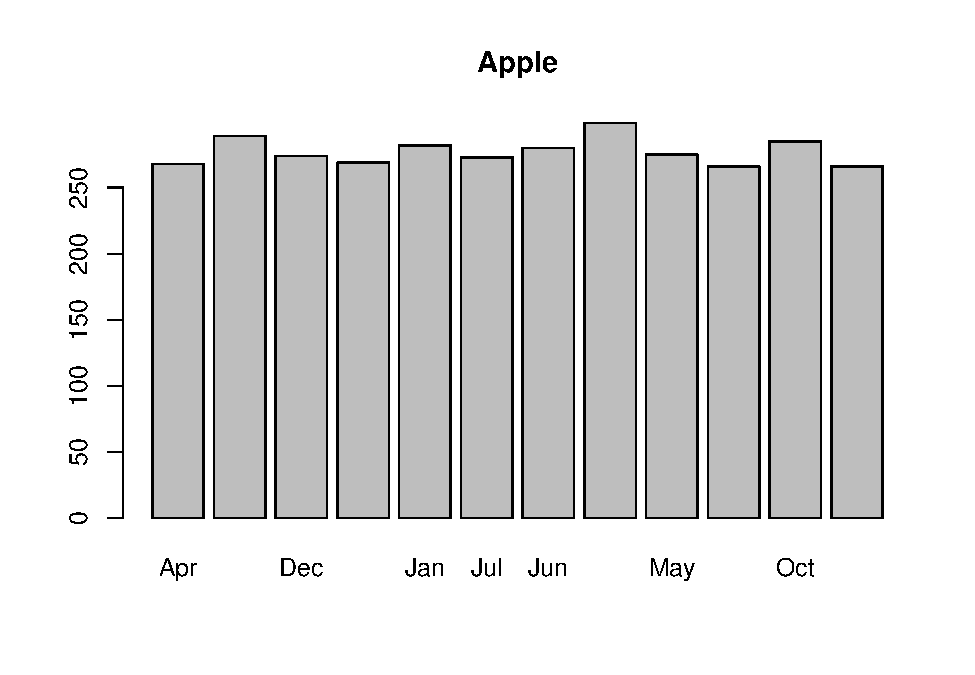
\includegraphics[width=0.7\linewidth]{Lab_3_files/figure-latex/unnamed-chunk-34-1} \end{center}

\begin{Shaded}
\begin{Highlighting}[]
\NormalTok{x.apple =}\StringTok{ }\KeywordTok{table}\NormalTok{(}\KeywordTok{strftime}\NormalTok{(apple_data}\OperatorTok{$}\NormalTok{Date, }\StringTok{"%b"}\NormalTok{))}
\NormalTok{x.msft =}\StringTok{ }\KeywordTok{table}\NormalTok{(}\KeywordTok{strftime}\NormalTok{(msft_data}\OperatorTok{$}\NormalTok{Date, }\StringTok{"%b"}\NormalTok{))}
\NormalTok{x.google =}\StringTok{ }\KeywordTok{table}\NormalTok{(}\KeywordTok{strftime}\NormalTok{(google_data}\OperatorTok{$}\NormalTok{Date, }\StringTok{"%b"}\NormalTok{))}

\NormalTok{dat.stoc.month =}\StringTok{ }\KeywordTok{rbind}\NormalTok{(x.apple, x.msft, x.google)}
\KeywordTok{row.names}\NormalTok{(dat.stoc.month) =}\StringTok{ }\KeywordTok{c}\NormalTok{(}\StringTok{"Apple"}\NormalTok{, }\StringTok{"Microsoft"}\NormalTok{, }\StringTok{"Google"}\NormalTok{)}
  
\KeywordTok{barplot}\NormalTok{(dat.stoc.month,}
        \DataTypeTok{beside =} \OtherTok{TRUE}\NormalTok{,}
        \DataTypeTok{main =} \StringTok{"Numarul de tranzactii lunare"}\NormalTok{,}
        \DataTypeTok{col =} \KeywordTok{c}\NormalTok{(}\StringTok{"brown3"}\NormalTok{, }\StringTok{"forestgreen"}\NormalTok{, }\StringTok{"royalblue"}\NormalTok{), }
        \DataTypeTok{legend.text=}\KeywordTok{c}\NormalTok{(}\StringTok{"Apple"}\NormalTok{, }\StringTok{"Microsoft"}\NormalTok{, }\StringTok{"Google"}\NormalTok{),}
        \DataTypeTok{args.legend=}\KeywordTok{list}\NormalTok{(}\DataTypeTok{x=}\StringTok{"bottomright"}\NormalTok{, }\DataTypeTok{bty =} \StringTok{"n"}\NormalTok{),}
        \DataTypeTok{xlim =} \KeywordTok{c}\NormalTok{(}\DecValTok{0}\NormalTok{, }\DecValTok{58}\NormalTok{),}
        \DataTypeTok{cex.names =} \FloatTok{0.7}\NormalTok{, }
        \DataTypeTok{cex.axis =} \FloatTok{0.7}\NormalTok{)}
\end{Highlighting}
\end{Shaded}

\begin{center}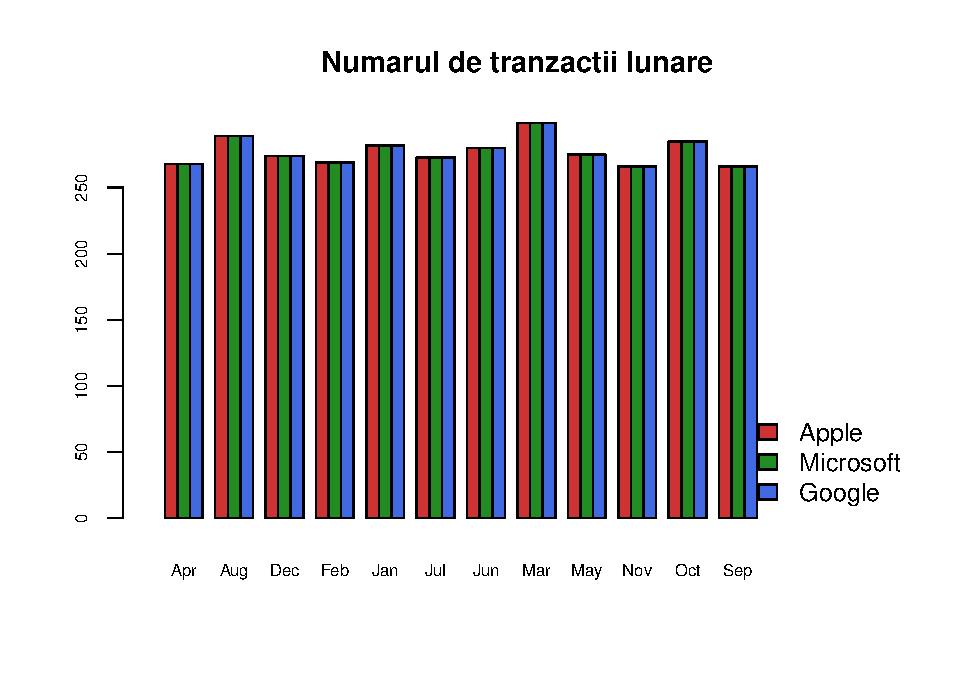
\includegraphics[width=0.7\linewidth]{Lab_3_files/figure-latex/unnamed-chunk-35-1} \end{center}

\subsection{Histograma}\label{histograma}

\emph{Histograma} este un exemplu de metodă neparametrică de estimare a
densității de probabilitate. Fie \(X_1, X_2, \ldots, X_n\) un eșantion
de talie \(n\) dintr-o populație cu densitate de probabilitate \(f\).
Fără a restrânge generalitatea putem să presupunem că \(X_i\in[0,1]\)
(în caz contrar putem scala observațiile la acest interval).

Fie \(m\) un număr natural și să considerăm diviziunea intervalului
\([0,1]\) (fiecare subinterval din diviziune se numește \emph{bin}):

\[
  B_1 = \left[0, \frac{1}{m}\right), \, B_2 = \left[\frac{1}{m}, \frac{2}{m}\right),\cdots,\, B_m = \left[\frac{m-1}{m}, 1\right].
\]

Notăm cu \(h = \frac{1}{m}\) lungimea bin-urilor,
\(p_j = \mathbb{P}(X_i\in B_j) = \int_{B_j}f(t)\,dt\) probabilitatea ca
o observație să pice în subintervalul \(B_j\) și
\(\hat{p}_j = \frac{1}{n}\sum_{i = 1}^{n}\mathbf{1}_{\left\{X_i \in B_j\right\}}\)
numărul de observații, din cele \(n\), care se află în intervalul
\(B_j\). Atunci estimatorul \emph{histogramă} este dat de

\[
  \hat{f}_n(x) = \left\{\begin{array}{llll}
            \frac{\hat{p}_1}{h}, & x\in B_1\\
            \frac{\hat{p}_2}{h}, & x\in B_2\\
            \vdots, & \vdots\\
            \frac{\hat{p}_m}{h}, & x\in B_m
  \end{array}\right.
\]

care scris sub formă compactă devine

\[
  \hat{f}_n(x) = \sum_{i=1}^{m} \frac{\hat{p}_i}{h} \mathbf{1}_{B_i}(x).
\]

Se poate observa că pentru \(m\) suficient de mare (\(h\) mic) și
\(x\in B_j\) avem

\[
  \mathbb{E}\left[\hat{f}_n(x)\right] = \mathbb{E}\left[\sum_{i=1}^{m} \frac{\hat{p}_i}{h} \mathbf{1}_{B_i}(x)\right]= \frac{\mathbb{E}\left[\hat{p}_j\right]}{h} = \frac{p_j}{h} = \frac{\int_{B_j}f(x)\,dx}{h}\approx \frac{f(x)h}{h} = f(x).
\]

Alegerea numărului de bin-uri și a mărimii acestora nu este o problemă
trivială. De exemplu, D. Scott propune o variantă de alegere a lui \(k\)
în articolul (Scott 1979). Un rezultat similar, dar mai robust, a fost
obținut de D. Freedman și P. Diaconis în (Freedman and Diaconis 1981).
Câteva dintre metodele de alegere a mărimii bin-ului sunt prezentate în
următoarea pagină de
\href{https://en.wikipedia.org/wiki/Histogram\#Number_of_bins_and_width}{Wikipedia}.

În R, funcția \texttt{hist()} este folosită pentru trasarea unei
histograme. Această funcție utilizează ca metodă predefinită de alegere
a mărimii bin-urilor, metoda lui Sturges (a se vedea articolul (Sturges
1926)).

\begin{rmdexercise}
Investigați cu ajutorul unei histograme cum este repartizat prețul
zilnic al celor trei stoc-uri în perioada 2008-2009.
\end{rmdexercise}

\begin{Shaded}
\begin{Highlighting}[]
\KeywordTok{par}\NormalTok{(}\DataTypeTok{mfrow =} \KeywordTok{c}\NormalTok{(}\DecValTok{1}\NormalTok{,}\DecValTok{3}\NormalTok{))}

\KeywordTok{hist}\NormalTok{(apple_data}\OperatorTok{$}\NormalTok{Close[}\KeywordTok{strftime}\NormalTok{(apple_data}\OperatorTok{$}\NormalTok{Date, }\StringTok{"%Y"}\NormalTok{) }\OperatorTok\StringTok{ }\KeywordTok{c}\NormalTok{(}\StringTok{"2008"}\NormalTok{, }\StringTok{"2009"}\NormalTok{)], }
     \DataTypeTok{probability =} \OtherTok{TRUE}\NormalTok{, }
     \DataTypeTok{col =} \StringTok{"grey80"}\NormalTok{,}
     \DataTypeTok{main =} \StringTok{"Repartitia pretului zilnic}\CharTok{\textbackslash{}n}\StringTok{ Apple"}\NormalTok{,}
     \DataTypeTok{xlab =} \StringTok{"Pret"}\NormalTok{,}
     \DataTypeTok{ylab =} \StringTok{"Densitatea"}\NormalTok{, }
     \DataTypeTok{cex.main =} \FloatTok{0.8}\NormalTok{)}

\KeywordTok{hist}\NormalTok{(msft_data}\OperatorTok{$}\NormalTok{Close[}\KeywordTok{strftime}\NormalTok{(msft_data}\OperatorTok{$}\NormalTok{Date, }\StringTok{"%Y"}\NormalTok{) }\OperatorTok\StringTok{ }\KeywordTok{c}\NormalTok{(}\StringTok{"2008"}\NormalTok{, }\StringTok{"2009"}\NormalTok{)], }
     \DataTypeTok{probability =} \OtherTok{TRUE}\NormalTok{, }
     \DataTypeTok{breaks =} \StringTok{"FD"}\NormalTok{,}
     \DataTypeTok{col =} \StringTok{"grey80"}\NormalTok{,}
     \DataTypeTok{main =} \StringTok{"Repartitia pretului zilnic}\CharTok{\textbackslash{}n}\StringTok{ Microsoft"}\NormalTok{,}
     \DataTypeTok{xlab =} \StringTok{"Pret"}\NormalTok{,}
     \DataTypeTok{ylab =} \StringTok{"Densitatea"}\NormalTok{, }
     \DataTypeTok{cex.main =} \FloatTok{0.8}\NormalTok{)}

\KeywordTok{hist}\NormalTok{(google_data}\OperatorTok{$}\NormalTok{Close[}\KeywordTok{strftime}\NormalTok{(google_data}\OperatorTok{$}\NormalTok{Date, }\StringTok{"%Y"}\NormalTok{) }\OperatorTok\StringTok{ }\KeywordTok{c}\NormalTok{(}\StringTok{"2008"}\NormalTok{, }\StringTok{"2009"}\NormalTok{)], }
     \DataTypeTok{probability =} \OtherTok{TRUE}\NormalTok{, }
     \DataTypeTok{breaks =} \KeywordTok{seq}\NormalTok{(}\DecValTok{100}\NormalTok{, }\DecValTok{450}\NormalTok{, }\DecValTok{25}\NormalTok{),}
     \DataTypeTok{col =} \StringTok{"grey80"}\NormalTok{,}
     \DataTypeTok{main =} \StringTok{"Repartitia pretului zilnic}\CharTok{\textbackslash{}n}\StringTok{ Google"}\NormalTok{,}
     \DataTypeTok{xlab =} \StringTok{"Pret"}\NormalTok{,}
     \DataTypeTok{ylab =} \StringTok{"Densitatea"}\NormalTok{, }
     \DataTypeTok{cex.main =} \FloatTok{0.8}\NormalTok{)}
\end{Highlighting}
\end{Shaded}

\begin{center}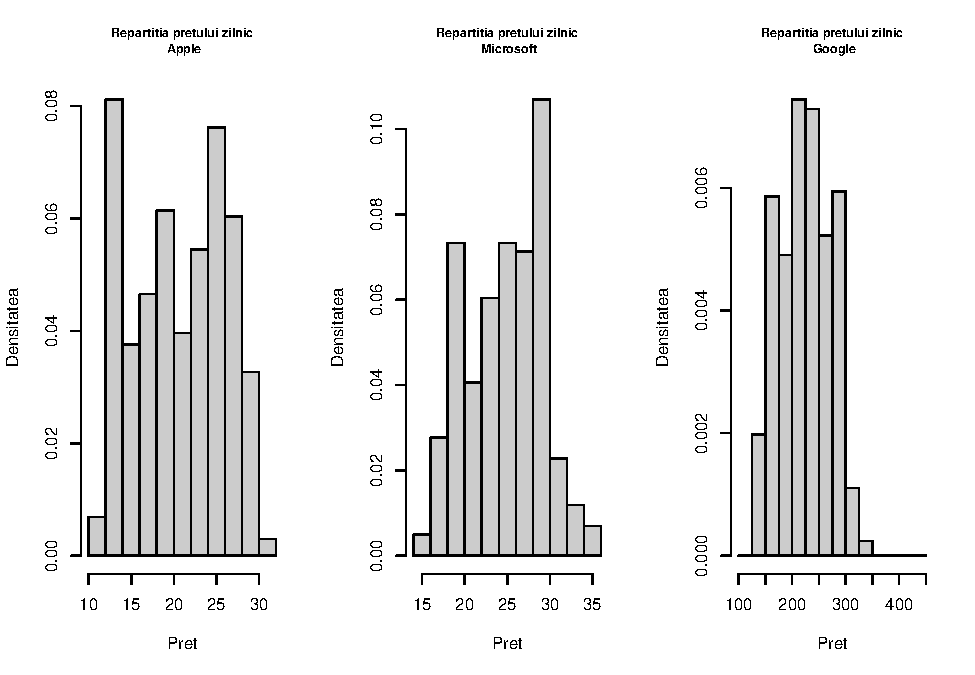
\includegraphics[width=0.7\linewidth]{Lab_3_files/figure-latex/unnamed-chunk-37-1} \end{center}

\begin{rmdexercise}
Investigați cu ajutorul unei histograme cum este repartizată
rentabilitatea zilnică și respectiv lunară al celor trei stoc-uri pentru
perioada 2008-2009.
\end{rmdexercise}

\begin{rmdexercise}
Considerați setul de date \texttt{mtcars}. Investigați cu ajutorul unei
histograme cum este repartizată variabila \texttt{hp}. Trasați prin
drepte verticale de culori diferite media și respectiv mediana datelor.
\end{rmdexercise}

\begin{Shaded}
\begin{Highlighting}[]
\KeywordTok{par}\NormalTok{(}\DataTypeTok{mfrow =} \KeywordTok{c}\NormalTok{(}\DecValTok{1}\NormalTok{,}\DecValTok{2}\NormalTok{))}

\KeywordTok{hist}\NormalTok{(mtcars}\OperatorTok{$}\NormalTok{hp, }\DataTypeTok{freq =} \OtherTok{FALSE}\NormalTok{,}
     \DataTypeTok{main =} \StringTok{"Horepower - HP}\CharTok{\textbackslash{}n}\StringTok{ (default)"}\NormalTok{, }
     \DataTypeTok{xlab=}\StringTok{"HP"}\NormalTok{)}

\KeywordTok{hist}\NormalTok{(mtcars}\OperatorTok{$}\NormalTok{hp, }\DataTypeTok{freq =} \OtherTok{FALSE}\NormalTok{,}
     \DataTypeTok{breaks=}\KeywordTok{seq}\NormalTok{(}\DecValTok{0}\NormalTok{,}\DecValTok{400}\NormalTok{,}\DecValTok{25}\NormalTok{),}
     \DataTypeTok{col=}\StringTok{"gray"}\NormalTok{,}
     \DataTypeTok{main=}\StringTok{"Horsepower - HP}\CharTok{\textbackslash{}n}\StringTok{ (marimea bin-ului 25)"}\NormalTok{,}
     \DataTypeTok{xlab=}\StringTok{"HP"}\NormalTok{)}

\KeywordTok{abline}\NormalTok{(}\DataTypeTok{v=}\KeywordTok{c}\NormalTok{(}\KeywordTok{mean}\NormalTok{(mtcars}\OperatorTok{$}\NormalTok{hp), }\KeywordTok{median}\NormalTok{(mtcars}\OperatorTok{$}\NormalTok{hp)), }
       \DataTypeTok{lty=}\KeywordTok{c}\NormalTok{(}\DecValTok{2}\NormalTok{,}\DecValTok{3}\NormalTok{), }\DataTypeTok{lwd=}\DecValTok{2}\NormalTok{)}
\KeywordTok{legend}\NormalTok{(}\StringTok{"topright"}\NormalTok{, }\DataTypeTok{legend=}\KeywordTok{c}\NormalTok{(}\StringTok{"media HP"}\NormalTok{,}\StringTok{"mediana HP"}\NormalTok{),}
       \DataTypeTok{lty=}\KeywordTok{c}\NormalTok{(}\DecValTok{2}\NormalTok{,}\DecValTok{3}\NormalTok{), }\DataTypeTok{lwd=}\DecValTok{2}\NormalTok{,}
       \DataTypeTok{bty =} \StringTok{"n"}\NormalTok{)}
\end{Highlighting}
\end{Shaded}

\begin{center}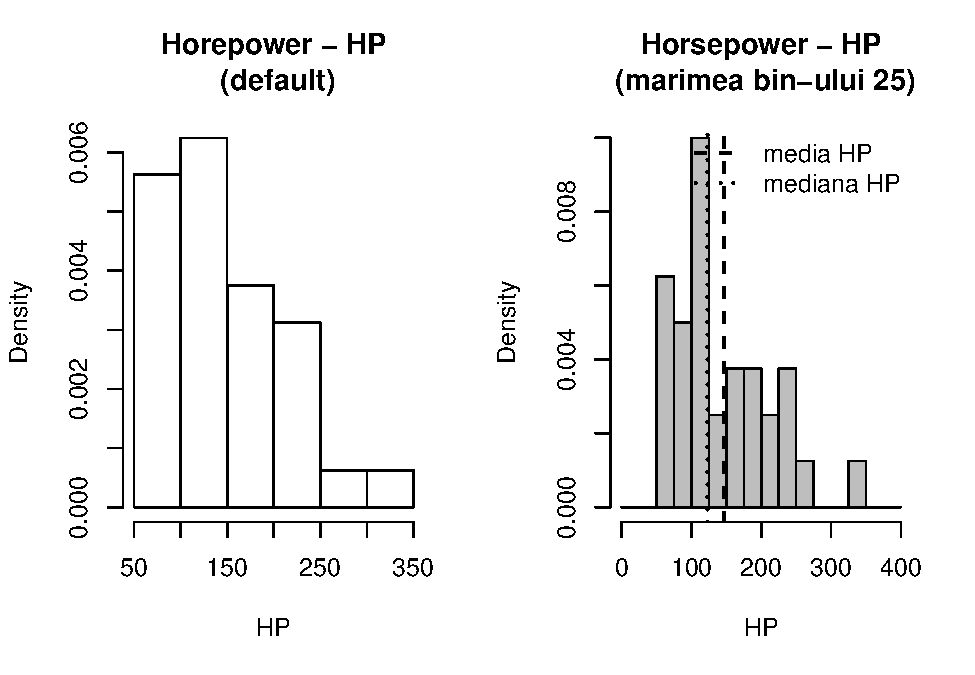
\includegraphics[width=0.7\linewidth]{Lab_3_files/figure-latex/unnamed-chunk-40-1} \end{center}

\begin{rmdexercise}
Să presupunem că în fișierul
\href{\%22dataIn/studFMI.txt\%22}{studFMI.txt} am stocat date privind
sexul (f/h), înălțimea (în cm) și greutatea (în kg) a studenților de
master de la Facultatea de Matematică și Informatică. Vrem să
investigăm, trasând pe același grafic, cum este repartizată înălțimea și
respectiv greutatea studenților în funcție de sex.
\end{rmdexercise}

Începem prin a citi datele din fișier:

\begin{Shaded}
\begin{Highlighting}[]
\NormalTok{stud =}\StringTok{ }\KeywordTok{read.table}\NormalTok{(}\StringTok{"dataIn/studFMI.txt"}\NormalTok{, }\DataTypeTok{header =} \OtherTok{TRUE}\NormalTok{)}
\KeywordTok{str}\NormalTok{(stud)}
\StringTok{'data.frame'}\OperatorTok{:}\StringTok{   }\DecValTok{97}\NormalTok{ obs. of  }\DecValTok{3}\NormalTok{ variables}\OperatorTok{:}
\StringTok{ }\ErrorTok{$}\StringTok{ }\NormalTok{sex   }\OperatorTok{:}\StringTok{ }\NormalTok{Factor w}\OperatorTok{/}\StringTok{ }\DecValTok{2}\NormalTok{ levels }\StringTok{"f"}\NormalTok{,}\StringTok{"h"}\OperatorTok{:}\StringTok{ }\DecValTok{2} \DecValTok{2} \DecValTok{1} \DecValTok{1} \DecValTok{2} \DecValTok{1} \DecValTok{2} \DecValTok{2} \DecValTok{2} \DecValTok{2}\NormalTok{ ...}
 \OperatorTok{$}\StringTok{ }\NormalTok{height}\OperatorTok{:}\StringTok{ }\NormalTok{int  }\DecValTok{168} \DecValTok{177} \DecValTok{164} \DecValTok{166} \DecValTok{165} \DecValTok{150} \DecValTok{186} \DecValTok{185} \DecValTok{181} \DecValTok{188}\NormalTok{ ...}
 \OperatorTok{$}\StringTok{ }\NormalTok{weight}\OperatorTok{:}\StringTok{ }\NormalTok{int  }\DecValTok{69} \DecValTok{73} \DecValTok{53} \DecValTok{57} \DecValTok{60} \DecValTok{42} \DecValTok{74} \DecValTok{83} \DecValTok{77} \DecValTok{72}\NormalTok{ ...}
\KeywordTok{head}\NormalTok{(stud)}
\NormalTok{  sex height weight}
\DecValTok{1}\NormalTok{   h    }\DecValTok{168}     \DecValTok{69}
\DecValTok{2}\NormalTok{   h    }\DecValTok{177}     \DecValTok{73}
\DecValTok{3}\NormalTok{   f    }\DecValTok{164}     \DecValTok{53}
\DecValTok{4}\NormalTok{   f    }\DecValTok{166}     \DecValTok{57}
\DecValTok{5}\NormalTok{   h    }\DecValTok{165}     \DecValTok{60}
\DecValTok{6}\NormalTok{   f    }\DecValTok{150}     \DecValTok{42}
\end{Highlighting}
\end{Shaded}

Separăm înălțimea (greutatea este exercițiu!) bărbaților și a femeilor:

\begin{Shaded}
\begin{Highlighting}[]
\CommentTok{# h vine de la hommes iar f de la femmes}
\NormalTok{hm =}\StringTok{ }\NormalTok{stud}\OperatorTok{$}\NormalTok{height[stud}\OperatorTok{$}\NormalTok{sex }\OperatorTok{==}\StringTok{ "h"}\NormalTok{]}
\NormalTok{hf =}\StringTok{ }\NormalTok{stud}\OperatorTok{$}\NormalTok{height[stud}\OperatorTok{$}\NormalTok{sex }\OperatorTok{==}\StringTok{ "f"}\NormalTok{]}

\KeywordTok{par}\NormalTok{(}\DataTypeTok{mfrow =} \KeywordTok{c}\NormalTok{(}\DecValTok{1}\NormalTok{,}\DecValTok{2}\NormalTok{))}

\KeywordTok{hist}\NormalTok{(hm, }\DataTypeTok{freq =} \OtherTok{FALSE}\NormalTok{, }\DataTypeTok{col =} \KeywordTok{grey}\NormalTok{(}\FloatTok{0.8}\NormalTok{),}
     \DataTypeTok{main =} \StringTok{"Inaltimea barbatilor"}\NormalTok{, }
     \DataTypeTok{xlab =} \StringTok{"inaltimea"}\NormalTok{,}
     \DataTypeTok{ylab =} \StringTok{"densitatea"}\NormalTok{)}
\NormalTok{tm =}\StringTok{ }\KeywordTok{seq}\NormalTok{(}\KeywordTok{min}\NormalTok{(hm)}\OperatorTok{-}\DecValTok{5}\NormalTok{, }\KeywordTok{max}\NormalTok{(hm)}\OperatorTok{+}\DecValTok{5}\NormalTok{, }\DataTypeTok{length.out =} \DecValTok{100}\NormalTok{)}
\KeywordTok{lines}\NormalTok{(tm, }\KeywordTok{dnorm}\NormalTok{(tm, }\KeywordTok{mean}\NormalTok{(hm), }\KeywordTok{sd}\NormalTok{(hm)), }
      \DataTypeTok{lty =} \DecValTok{2}\NormalTok{, }\DataTypeTok{lwd =} \DecValTok{2}\NormalTok{)}

\KeywordTok{hist}\NormalTok{(hf, }\DataTypeTok{freq =} \OtherTok{FALSE}\NormalTok{, }\DataTypeTok{col =} \KeywordTok{grey}\NormalTok{(}\FloatTok{0.8}\NormalTok{),}
     \DataTypeTok{main =} \StringTok{"Inaltimea femeilor"}\NormalTok{, }
     \DataTypeTok{xlab =} \StringTok{"inaltimea"}\NormalTok{,}
     \DataTypeTok{ylab =} \StringTok{"densitatea"}\NormalTok{)}
\NormalTok{tf =}\StringTok{ }\KeywordTok{seq}\NormalTok{(}\KeywordTok{min}\NormalTok{(hf)}\OperatorTok{-}\DecValTok{5}\NormalTok{, }\KeywordTok{max}\NormalTok{(hf)}\OperatorTok{+}\DecValTok{5}\NormalTok{, }\DataTypeTok{length.out =} \DecValTok{100}\NormalTok{)}
\KeywordTok{lines}\NormalTok{(tf, }\KeywordTok{dnorm}\NormalTok{(tf, }\KeywordTok{mean}\NormalTok{(hf), }\KeywordTok{sd}\NormalTok{(hf)), }
      \DataTypeTok{lty =} \DecValTok{2}\NormalTok{, }\DataTypeTok{lwd =} \DecValTok{2}\NormalTok{)}
\end{Highlighting}
\end{Shaded}

\begin{center}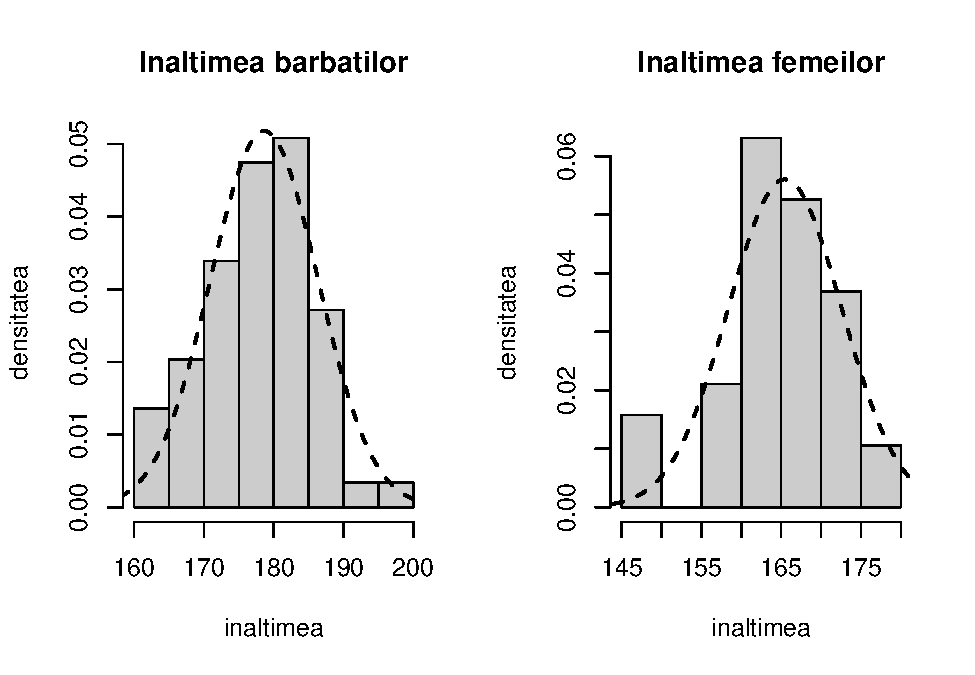
\includegraphics[width=0.8\linewidth]{Lab_3_files/figure-latex/unnamed-chunk-43-1} \end{center}

Reprezentăm repartiția înălțimilor luate împreună și evidențiem mixtura
celor două repartiții după sex:

\begin{Shaded}
\begin{Highlighting}[]
\NormalTok{height =}\StringTok{ }\NormalTok{stud}\OperatorTok{$}\NormalTok{height}

\KeywordTok{hist}\NormalTok{(height, }\DataTypeTok{proba =} \OtherTok{TRUE}\NormalTok{, }
     \DataTypeTok{breaks=}\DecValTok{25}\NormalTok{, }
     \DataTypeTok{col =} \KeywordTok{grey}\NormalTok{(}\FloatTok{0.8}\NormalTok{), }
     \DataTypeTok{main =} \StringTok{"Inaltimea barbatilor si a femeilor"}\NormalTok{,}
     \DataTypeTok{xlab =} \StringTok{"inaltimea"}\NormalTok{,}
     \DataTypeTok{ylab =} \StringTok{"densitatea"}\NormalTok{,}
     \DataTypeTok{ylim =} \KeywordTok{c}\NormalTok{(}\DecValTok{0}\NormalTok{, }\FloatTok{0.05}\NormalTok{))}

\NormalTok{t <-}\StringTok{ }\KeywordTok{seq}\NormalTok{(}\DecValTok{145}\NormalTok{,}\DecValTok{200}\NormalTok{,}\DataTypeTok{length=}\DecValTok{100}\NormalTok{)}

\NormalTok{x1 <-}\StringTok{ }\KeywordTok{dnorm}\NormalTok{(t,}\KeywordTok{mean}\NormalTok{(hf),}\KeywordTok{sd}\NormalTok{(hf))}
\NormalTok{x2 <-}\StringTok{ }\KeywordTok{dnorm}\NormalTok{(t,}\KeywordTok{mean}\NormalTok{(hm),}\KeywordTok{sd}\NormalTok{(hm))}

\CommentTok{# proportia de femei (din nr de studenti)}
\NormalTok{pf <-}\StringTok{ }\KeywordTok{length}\NormalTok{(hf)}\OperatorTok{/}\KeywordTok{length}\NormalTok{(height)}

\CommentTok{# mixtura dintre rep inaltimilor f si h}
\NormalTok{x3 <-}\StringTok{ }\NormalTok{pf}\OperatorTok{*}\NormalTok{x1 }\OperatorTok{+}\StringTok{ }\NormalTok{(}\DecValTok{1}\OperatorTok{-}\NormalTok{pf)}\OperatorTok{*}\NormalTok{x2}

\KeywordTok{lines}\NormalTok{(t, x3, }\DataTypeTok{lwd =} \DecValTok{2}\NormalTok{)}

\KeywordTok{lines}\NormalTok{(t, pf}\OperatorTok{*}\NormalTok{x1, }\DataTypeTok{col =} \StringTok{"brown3"}\NormalTok{, }
      \DataTypeTok{lty =} \DecValTok{2}\NormalTok{, }\DataTypeTok{lwd =} \DecValTok{2}\NormalTok{)}
\KeywordTok{lines}\NormalTok{(t, (}\DecValTok{1}\OperatorTok{-}\NormalTok{pf)}\OperatorTok{*}\NormalTok{x2, }\DataTypeTok{col =} \StringTok{"royalblue"}\NormalTok{, }
      \DataTypeTok{lty =} \DecValTok{2}\NormalTok{, }\DataTypeTok{lwd =} \DecValTok{2}\NormalTok{)}

\KeywordTok{legend}\NormalTok{(}\StringTok{"topright"}\NormalTok{, }\KeywordTok{c}\NormalTok{(}\StringTok{"femei"}\NormalTok{,}\StringTok{"barbati"}\NormalTok{), }
       \DataTypeTok{col =} \KeywordTok{c}\NormalTok{(}\StringTok{"brown3"}\NormalTok{,}\StringTok{"royalblue"}\NormalTok{), }
       \DataTypeTok{lty =} \DecValTok{2}\NormalTok{, }\DataTypeTok{lwd =} \DecValTok{2}\NormalTok{, }
       \DataTypeTok{bty =} \StringTok{"n"}\NormalTok{)}
\end{Highlighting}
\end{Shaded}

\begin{center}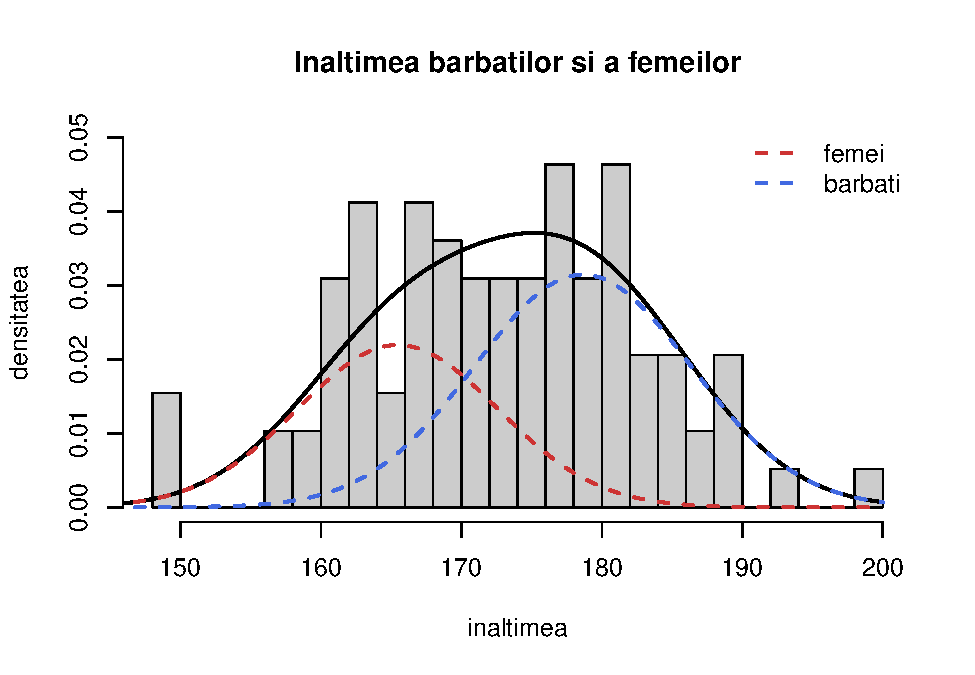
\includegraphics[width=0.8\linewidth]{Lab_3_files/figure-latex/unnamed-chunk-44-1} \end{center}

\subsection{Boxplot}\label{boxplot}

Una dintre metodele grafice des întâlnite în vizualizarea datelor
(cantitative) unidimensionale este \emph{boxplot}-ul (eng. \emph{box and
whisker plot} - cutia cu mustăți). Această metodă grafică descriptivă
este folosită în principal pentru a investiga forma repartiției
(simetrică sau asimetrică) datelor dar și variabilitatea acestora precum
și pentru detectarea și ilustrarea schimbărilor de locație și variație
între diferitele grupuri de date.

După cum putem vedea și în figura de mai jos, cutia este definită, de la
stânga la dreapta (sau de jos în sus în funcție de cum este reprezentat
boxplot-ul: orizontal sau vertical), de prima cuartilă \(Q_1\) și de a
treia curatilă \(Q_3\) ceea ce înseamnă că \(50\%\) dintre observații se
află în interiorul cutiei. Linia din interiorul cutiei este determinată
de mediană sau a doua cuartilă \(Q_2\).

Mustățile care pornesc de o parte și de alta a cutiei sunt determinate
astfel (vom folosi conveția folosită de John Tukey în (J. 1977, pag.
40-56)): mustața din stânga este determinată de cea mai mică observație
mai mare decât \(Q_1-1.5 IQR\) iar cea din dreapta de cea mai mare
observație din setul de date mai mică decât \(Q_3+1.5IQR\), unde
\(IQR = Q_3-Q_1\) este distanța dintre cuartile (\emph{interquartile
range}).

Valorile observațiilor din setul de date care sunt sau prea mici sau
prea mari se numesc valori aberante (\emph{outliers}) și conform lui
Tukey sunt definite astfel: \emph{valori strict aberante} care se află
la \(3IQR\) deasupra celei de-a treia curtilă \(Q_3\) sau la \(3IQR\)
sub prima cuartilă (\(x<Q_1-3IQR\) sau \(x>Q_3+3IQR\)) și \emph{valori
potențial aberante} care se află la \(1.5IQR\) deasupra celei de-a treia
curtilă \(Q_3\) sau la \(1.5IQR\) sub prima cuartilă (\(x<Q_1-1.5IQR\)
sau \(x>Q_3+1.5IQR\)).

\begin{center}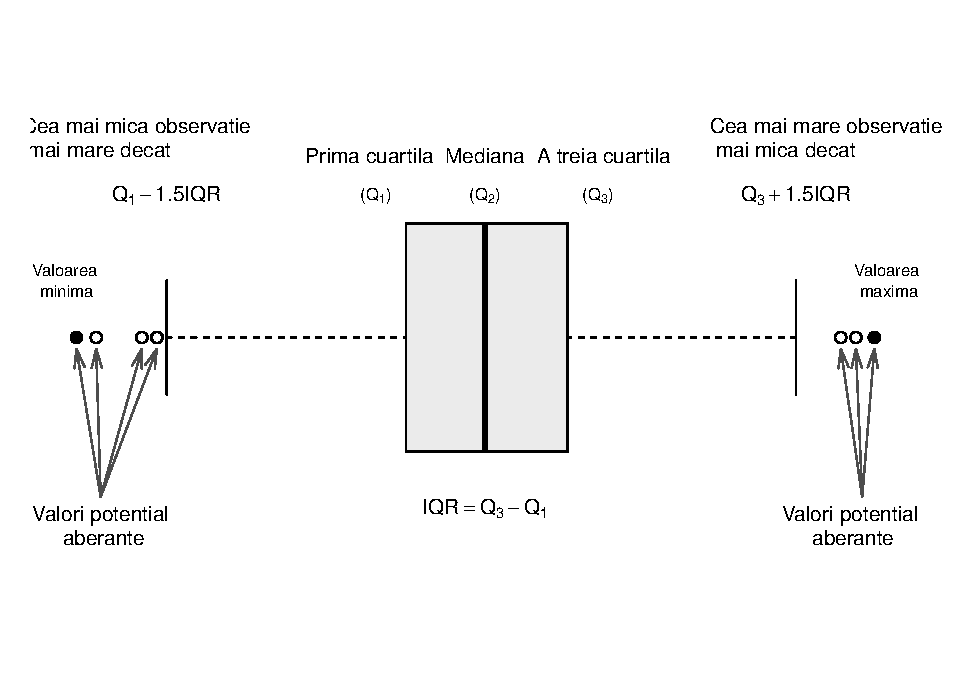
\includegraphics[width=0.7\linewidth]{Lab_3_files/figure-latex/unnamed-chunk-45-1} \end{center}

În R metoda grafică boxplot se poate trasa cu ajutorul funcției
\texttt{boxplot()}. Aceasta primește ca argumente sau un vector de
observații numerice \texttt{x} atunci când dorim să ilustrăm repartiția
unei variabile sau o formulă de tipul \texttt{y\textasciitilde{}grup},
unde \texttt{y} este un vector numeric care va fi împărțit în funcție de
variabila discretă \texttt{grup}, atunci când vrem să comparăm aceeași
variabilă numerică în funcție de una discretă (calitatăvă). Pentru mai
multe informații tastați \texttt{?boxplot}.

\begin{rmdexercise}
Considerați setul de date \texttt{mtcars}. Investigați cu ajutorul unui
boxplot cum variază greutatea mașinilor, variabila \texttt{wt}, în
funcție de numărul de cilindrii \texttt{cyl}. Afișați numele mașinilor
care prezintă potențiale valori aberante. Aceeași cerință pentru
perechile \texttt{mpg} - \texttt{cyl}, \texttt{hp} - \texttt{cyl} și
\texttt{hp} - \texttt{am}.
\end{rmdexercise}

\begin{Shaded}
\begin{Highlighting}[]
\KeywordTok{par}\NormalTok{(}\DataTypeTok{bty =} \StringTok{"n"}\NormalTok{)}
\NormalTok{bp =}\StringTok{ }\KeywordTok{boxplot}\NormalTok{(mtcars}\OperatorTok{$}\NormalTok{wt }\OperatorTok{~}\StringTok{ }\NormalTok{mtcars}\OperatorTok{$}\NormalTok{cyl,}
             \DataTypeTok{xlab =} \StringTok{"Numar de cilindrii"}\NormalTok{, }
             \DataTypeTok{ylab =} \StringTok{"Greutate (in tone)"}\NormalTok{,}
             \DataTypeTok{col =} \StringTok{"grey80"}\NormalTok{,}
             \DataTypeTok{main =} \StringTok{"Setul de date mtcars: greutate vs numar cilindrii"}\NormalTok{)}

\NormalTok{cars =}\StringTok{ }\NormalTok{mtcars[mtcars}\OperatorTok{$}\NormalTok{cyl }\OperatorTok{==}\StringTok{ }\DecValTok{8}\NormalTok{, ]}
\NormalTok{cars.names =}\StringTok{ }\KeywordTok{rownames}\NormalTok{(cars)[}\KeywordTok{which}\NormalTok{(cars}\OperatorTok{$}\NormalTok{wt }\OperatorTok\StringTok{ }\NormalTok{bp}\OperatorTok{$}\NormalTok{out)]}

\KeywordTok{text}\NormalTok{(}\KeywordTok{c}\NormalTok{(}\DecValTok{3}\NormalTok{,}\DecValTok{3}\NormalTok{,}\FloatTok{2.4}\NormalTok{)}\OperatorTok{+}\FloatTok{0.3}\NormalTok{, bp}\OperatorTok{$}\NormalTok{out, cars.names, }\DataTypeTok{cex =} \FloatTok{0.6}\NormalTok{)}
\KeywordTok{text}\NormalTok{( }\KeywordTok{c}\NormalTok{(}\DecValTok{1}\OperatorTok{:}\KeywordTok{length}\NormalTok{(}\KeywordTok{unique}\NormalTok{(mtcars}\OperatorTok{$}\NormalTok{cyl))) , }
\NormalTok{      bp}\OperatorTok{$}\NormalTok{stats[}\KeywordTok{nrow}\NormalTok{(bp}\OperatorTok{$}\NormalTok{stats) , ] }\OperatorTok{+}\StringTok{ }\FloatTok{0.5}\NormalTok{ , }
      \KeywordTok{paste}\NormalTok{(}\StringTok{"n = "}\NormalTok{, }\KeywordTok{table}\NormalTok{(mtcars}\OperatorTok{$}\NormalTok{cyl),}\DataTypeTok{sep=}\StringTok{""}\NormalTok{),}
      \DataTypeTok{cex =} \FloatTok{0.8}\NormalTok{)}
\end{Highlighting}
\end{Shaded}

\begin{center}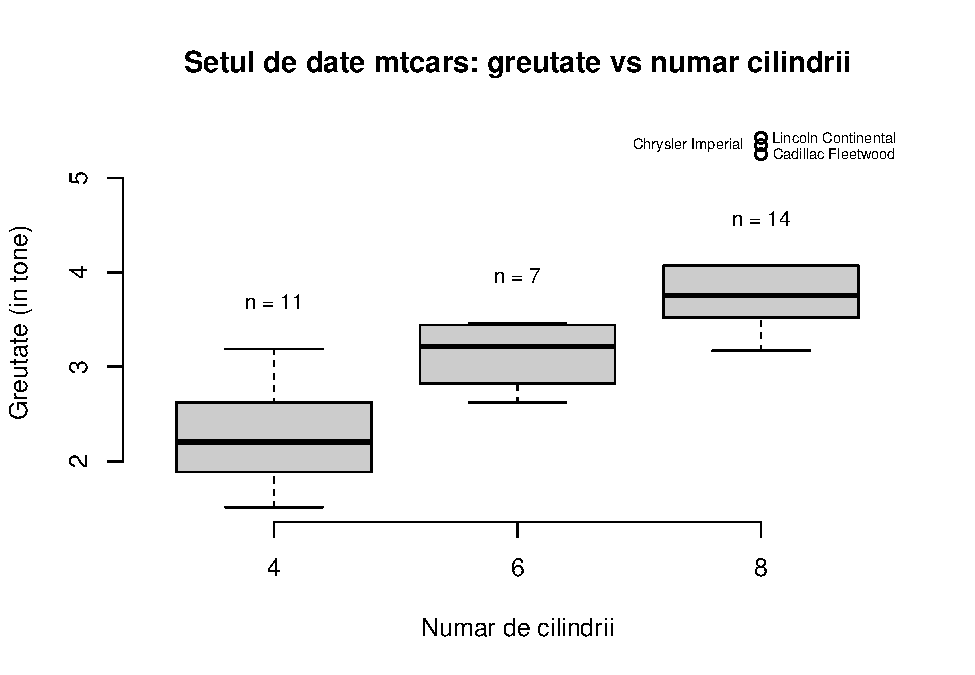
\includegraphics[width=0.7\linewidth]{Lab_3_files/figure-latex/unnamed-chunk-47-1} \end{center}

Numele mașinilor care au o greutate potențial aberantă este Cadillac
Fleetwood, Lincoln Continental, Chrysler Imperial.

\begin{rmdexercise}
Considerați stoc-urile firmelor Apple, Microsoft și Google. Investigați
cu ajutorul unui boxplot cum variază rentabilitatea zilnică a
stoc-urilor pentru fiecare firmă. Dar rentabilitatea lunară ajustată ?
\end{rmdexercise}

\begin{Shaded}
\begin{Highlighting}[]
\NormalTok{dat.stoc.daily =}\StringTok{ }\KeywordTok{data.frame}\NormalTok{(}\DataTypeTok{stock =} \KeywordTok{rep}\NormalTok{(}\KeywordTok{c}\NormalTok{(}\StringTok{"Apple"}\NormalTok{, }\StringTok{"Microsoft"}\NormalTok{, }\StringTok{"Google"}\NormalTok{), }
                                        \DataTypeTok{each =} \KeywordTok{c}\NormalTok{(}\KeywordTok{length}\NormalTok{(apple_ret_s_daily), }
                                                 \KeywordTok{length}\NormalTok{(msft_ret_s_daily),}
                                                 \KeywordTok{length}\NormalTok{(google_ret_s_daily))),}
                            \DataTypeTok{ret.day =} \KeywordTok{c}\NormalTok{(apple_ret_s_daily, }
\NormalTok{                                        msft_ret_s_daily, }
\NormalTok{                                        google_ret_s_daily))}

\KeywordTok{par}\NormalTok{(}\DataTypeTok{bty =} \StringTok{"n"}\NormalTok{)}
\NormalTok{bp =}\StringTok{ }\KeywordTok{boxplot}\NormalTok{(dat.stoc.daily}\OperatorTok{$}\NormalTok{ret.day }\OperatorTok{~}\StringTok{ }\NormalTok{dat.stoc.daily}\OperatorTok{$}\NormalTok{stock,}
             \DataTypeTok{xlab =} \StringTok{""}\NormalTok{, }
             \DataTypeTok{ylab =} \StringTok{"Rentabilitatea zilnica"}\NormalTok{,}
             \DataTypeTok{col =} \KeywordTok{c}\NormalTok{(}\StringTok{"brown3"}\NormalTok{, }\StringTok{"royalblue"}\NormalTok{, }\StringTok{"forestgreen"}\NormalTok{),}
             \DataTypeTok{main =} \StringTok{"Rentabilitatea zilnica pentru cele trei stoc-uri"}\NormalTok{,}
             \DataTypeTok{cex.main =} \FloatTok{0.8}\NormalTok{)}
\end{Highlighting}
\end{Shaded}

\begin{center}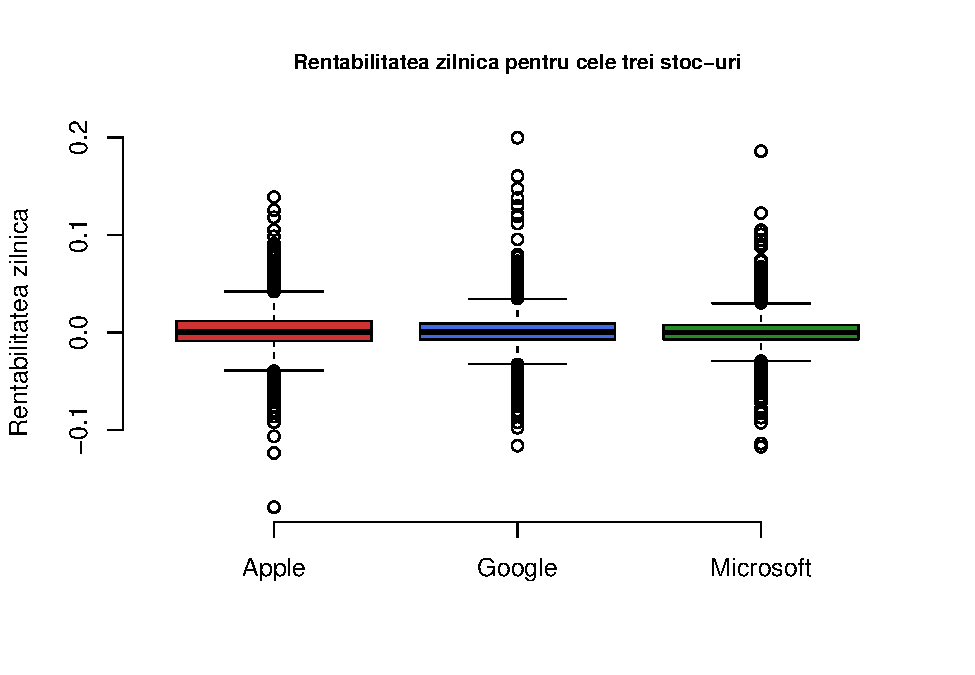
\includegraphics[width=0.7\linewidth]{Lab_3_files/figure-latex/unnamed-chunk-49-1} \end{center}

\begin{Shaded}
\begin{Highlighting}[]
\NormalTok{dat.stoc.monthly =}\StringTok{ }\KeywordTok{data.frame}\NormalTok{(}\DataTypeTok{stock =} \KeywordTok{rep}\NormalTok{(}\KeywordTok{c}\NormalTok{(}\StringTok{"Apple"}\NormalTok{, }\StringTok{"Microsoft"}\NormalTok{, }\StringTok{"Google"}\NormalTok{), }
                                        \DataTypeTok{each =} \KeywordTok{c}\NormalTok{(}\KeywordTok{length}\NormalTok{(apple_ret_adj_monthly}\OperatorTok{$}\NormalTok{ret), }
                                                 \KeywordTok{length}\NormalTok{(msft_ret_adj_monthly}\OperatorTok{$}\NormalTok{ret),}
                                                 \KeywordTok{length}\NormalTok{(google_ret_adj_monthly}\OperatorTok{$}\NormalTok{ret))),}
                            \DataTypeTok{ret.month.adj =} \KeywordTok{c}\NormalTok{(apple_ret_adj_monthly}\OperatorTok{$}\NormalTok{ret, }
\NormalTok{                                        msft_ret_adj_monthly}\OperatorTok{$}\NormalTok{ret, }
\NormalTok{                                        google_ret_adj_monthly}\OperatorTok{$}\NormalTok{ret))}

\KeywordTok{par}\NormalTok{(}\DataTypeTok{bty =} \StringTok{"n"}\NormalTok{)}
\NormalTok{bp =}\StringTok{ }\KeywordTok{boxplot}\NormalTok{(dat.stoc.monthly}\OperatorTok{$}\NormalTok{ret.month.adj }\OperatorTok{~}\StringTok{ }\NormalTok{dat.stoc.monthly}\OperatorTok{$}\NormalTok{stock,}
             \DataTypeTok{xlab =} \StringTok{""}\NormalTok{, }
             \DataTypeTok{ylab =} \StringTok{"Rentabilitatea lunara"}\NormalTok{,}
             \DataTypeTok{col =} \KeywordTok{c}\NormalTok{(}\StringTok{"brown3"}\NormalTok{, }\StringTok{"royalblue"}\NormalTok{, }\StringTok{"forestgreen"}\NormalTok{),}
             \DataTypeTok{main =} \StringTok{"Rentabilitatea lunara pentru cele trei stoc-uri"}\NormalTok{,}
             \DataTypeTok{cex.main =} \FloatTok{0.8}\NormalTok{)}
\end{Highlighting}
\end{Shaded}

\begin{center}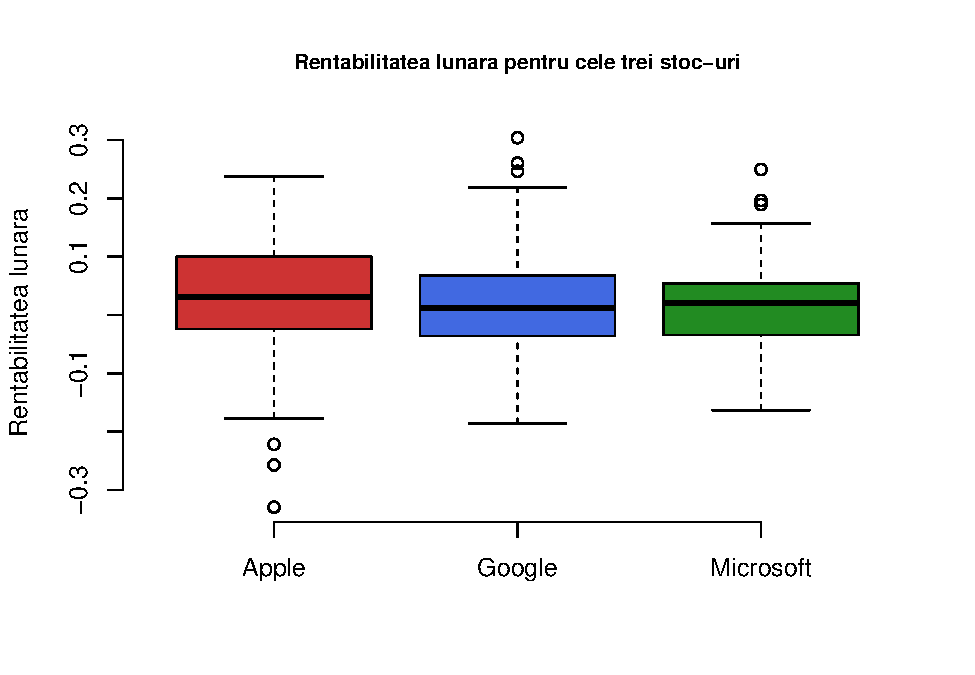
\includegraphics[width=0.7\linewidth]{Lab_3_files/figure-latex/unnamed-chunk-50-1} \end{center}

\section*{Referințe}\label{referinte}
\addcontentsline{toc}{section}{Referințe}

\hypertarget{refs}{}
\hypertarget{ref-FreedmanDiaconis1981}{}
Freedman, D., and P. Diaconis. 1981. ``On the Histogram as a Density
Estimator: \(L_2\) Theory.'' \emph{Z. Wahrscheinlichkeitstheorie Verw.
Gebiete} 57: 453--76.

\hypertarget{ref-Hyndman1996}{}
Hyndman, R. J., and Y Fan. 1996. ``Sample Quantiles in Statistical
Packages.'' \emph{American Statistician} 50: 361--65.

\hypertarget{ref-Tukey1977}{}
J., Tukey. 1977. \emph{Exploratory Data Analysis}. Addison-Wesley
Publishing Company.

\hypertarget{ref-Scott1979}{}
Scott, D. 1979. ``On Optimal and Data-Based Histograms.''
\emph{Biometrika} 66: 605--10.

\hypertarget{ref-Sturges1926}{}
Sturges, H. 1926. ``The Choice of a Class Interval.'' \emph{Journal of
the American Statistical Association} 65.


\end{document}
